\documentclass{article}
\usepackage{accsupp}
\usepackage{amsmath,amssymb,amstext,wasysym,enumerate}
\usepackage{array}
\usepackage{ctex}
\usepackage{diagbox}
\usepackage{enumitem}
\usepackage{fancyhdr}
\usepackage{float,abstract,booktabs,indentfirst}
\usepackage[a4paper, body={18cm,22cm}]{geometry}
\usepackage{graphicx}
\usepackage{hyperref}
\usepackage{listings}
\usepackage{makecell}
\usepackage{multirow}
\usepackage{subfigure}
\usepackage{tikz}
\usepackage{url}
\usepackage{xcolor}
\usetikzlibrary{shapes.geometric, arrows, positioning} % 添加 positioning 库


\renewcommand\arraystretch{1.4}
\setmonofont{Consolas}
\setlength{\parindent}{2em}

\pagestyle{fancy}
\fancyhead[L]{}
\fancyhead[R]{}
\fancyhead[C]{《数据库系统及其应用实践》课程实验报告}
\fancyfoot[C]{-\thepage-}
\renewcommand{\headrulewidth}{1.5pt}

\lstset{
    basicstyle=\ttfamily, 
    numbers=left, 
    numberstyle=\tiny, 
    keywordstyle=\color{blue},
    commentstyle=\color{gray}, 
    stringstyle=\color{red}, 
    frame=single,
    breaklines=true, 
    postbreak=\mbox{\textcolor{red}{$\hookrightarrow$}\space} 
}

\tikzset{
    base/.style={draw, align=center, minimum height=4ex, fill=white},
    block/.style={base, rectangle, text width=4cm, minimum height=10em, rounded corners},
    line/.style={draw, -latex'}
}

\begin{document}

\begin{center}
    \textbf{\LARGE{《数据库系统及其应用实践》课程实验报告}}

    \large{实验六: 查询处理 }

    \large{姓名: 武泽恺 \quad 学号: 10225101429}

\end{center}

\section{实验目标}
\begin{itemize}
    \item 学习MySQL数据库管理系统中显示查询执行计划的基本方法,理解查询处理的基本流程,并能够根据执行计划对查询性能进行分析和优化。
\end{itemize}

\section{实验要求}

\begin{itemize}
    \item 按照实验内容,依次完成每个实验步骤;
    \item 操作实验步骤时,需要理解该操作步骤的目的,预判操作的结果;当操作结果与预判不符时,及时向任课教师和助教咨询;
    \item 在实验报告中依次记录主要操作步骤的内容和结果(返回的消息或截图);
    \item 对实验中遇到的问题、解决方案及收获进行总结;
    \item 确保实验报告整洁、美观(注意字体、字号、对齐、截图大小和分页等;)
\end{itemize}

\section{实验内容}

我们使用EXPLAIN ANALYZE语句来查看查询执行计划,并对查询性能进行分析和优化。

同时,由于EXPLAIN ANALYZE查询出来的$cost$值是一个相对值,而$actual\_time$是一个绝对值,这可能不能直观反映对比估计代价和实际执行时间的差别。但是,我们发现,在$cost$和$actual\_time$后面都有一个字段$rows$,这个字段表示的是查询的行数。我们可以通过比对这个字段的值来对比估计代价和实际执行时间的差别。

为保证实验严谨性,我们每次测试前都会删除上一次测试建立的索引。

\subsection{TPCH测试}

我们首先进行TPC-H基准测试查询分析。

\subsubsection{测试语句一}

\begin{lstlisting}[language=sql]
EXPLAIN ANALYZE SELECT
l_returnflag,
l_linestatus,
sum( l_quantity ) AS sum_qty,
sum( l_extendedprice ) AS sum_base_price,
sum(
    l_extendedprice *(
    1-l_discount 
    )) AS sum_disc_price,
sum(
    l_extendedprice *(
    1-l_discount 
    )*(
    1+l_tax 
    )) AS sum_charge,
avg( l_quantity ) AS avg_qty,
avg( l_extendedprice ) AS avg_price,
avg( l_discount ) AS avg_disc,
count(*) AS count_order 
FROM
    lineitem 
WHERE
    l_shipdate <= DATE '1998-12-01' - INTERVAL '90' DAY 
GROUP BY
    l_returnflag,
    l_linestatus 
ORDER BY
    l_returnflag,
    l_linestatus;
\end{lstlisting}

得到结果:

\begin{lstlisting}
-> Sort: lineitem.l_returnflag, lineitem.l_linestatus  (actual time=3759..3759 rows=4 loops=1)
-> Table scan on <temporary>  (actual time=3759..3759 rows=4 loops=1)
    -> Aggregate using temporary table  (actual time=3759..3759 rows=4 loops=1)
        -> Filter: (lineitem.l_shipdate <= <cache>((DATE'1998-12-01' - interval '90' day)))  (cost=125656 rows=396583) (actual time=1.9..2537 rows=1.18e+6 loops=1)
            -> Table scan on lineitem  (cost=125656 rows=1.19e+6) (actual time=1.9..2461 rows=1.2e+6 loops=1)
\end{lstlisting}

查询耗时4.907s。

可以得知,查询的执行计划是先对lineitem表进行Table scan,然后对结果进行Filter,最后进行Aggregate操作。

我们可以看出,对于Table Scan来说,预估的行数会相对少一些,而实际的行数会相对多一些;而对于Filter和Aggregate操作来说,预估的行数会相对多一些,而实际的行数会相对少一些。

对于这个查询,我们可以对$l_orderkey,l_suppkey$字段建立索引,这两个字段是键,建立索引后可以加快查询速度。

\begin{lstlisting}
-> Sort: lineitem.l_returnflag, lineitem.l_linestatus  (actual time=3032..3032 rows=4 loops=1)
-> Table scan on <temporary>  (actual time=3032..3032 rows=4 loops=1)
    -> Aggregate using temporary table  (actual time=3032..3032 rows=4 loops=1)
        -> Filter: (lineitem.l_shipdate <= <cache>((DATE'1998-12-01' - interval '90' day)))  (cost=126258 rows=396583) (actual time=2.61..1811 rows=1.18e+6 loops=1)
            -> Table scan on lineitem  (cost=126258 rows=1.19e+6) (actual time=2.6..1734 rows=1.2e+6 loops=1)
\end{lstlisting}

耗时变为了3.032s,可以看到,建立索引后,速度上有所提升。

\subsubsection{测试语句二}

\begin{lstlisting}[language=sql]
EXPLAIN ANALYZE SELECT
s_acctbal,
s_name,
n_name,
p_partkey,
p_mfgr,
s_address,
s_phone,
s_comment 
FROM
part,
supplier,
partsupp,
nation,
region 
WHERE
p_partkey = ps_partkey 
AND s_suppkey = ps_suppkey 
AND p_size = 15 
AND p_type LIKE '%BRASS' 
AND s_nationkey = n_nationkey 
AND n_regionkey = r_regionkey 
AND r_name = 'EUROPE' 
AND ps_supplycost = (
SELECT
    min( ps_supplycost ) 
FROM
    partsupp,
    supplier,
    nation,
    region 
WHERE
    p_partkey = ps_partkey 
    AND s_suppkey = ps_suppkey 
    AND s_nationkey = n_nationkey 
    AND n_regionkey = r_regionkey 
    AND r_name = 'EUROPE' 
) 
ORDER BY
s_acctbal DESC,
n_name,
s_name,
p_partkey;
\end{lstlisting}

得到结果:

\begin{lstlisting}
-> Sort: supplier.s_acctbal DESC, nation.n_name, supplier.s_name, part.p_partkey  (actual time=16.7..16.7 rows=80 loops=1)
-> Stream results  (cost=5367 rows=1.96) (actual time=0.212..16.7 rows=80 loops=1)
    -> Nested loop inner join  (cost=5367 rows=1.96) (actual time=0.208..16.7 rows=80 loops=1)
        -> Nested loop inner join  (cost=4923 rows=19.6) (actual time=0.207..16.6 rows=80 loops=1)
            -> Nested loop inner join  (cost=4480 rows=19.6) (actual time=0.204..16.5 rows=80 loops=1)
                -> Inner hash join (no condition)  (cost=4067 rows=4.89) (actual time=0.126..9.91 rows=158 loops=1)
                    -> Filter: ((part.p_size = 15) and (part.p_type like '%BRASS'))  (cost=4066 rows=440) (actual time=0.079..9.85 rows=158 loops=1)
                        -> Table scan on part  (cost=4066 rows=39600) (actual time=0.0197..8.06 rows=40000 loops=1)
                    -> Hash
                        -> Filter: (region.r_name = 'EUROPE')  (cost=0.75 rows=1) (actual time=0.0364..0.0397 rows=1 loops=1)
                            -> Table scan on region  (cost=0.75 rows=5) (actual time=0.0317..0.0357 rows=5 loops=1)
                -> Filter: (partsupp.ps_supplycost = (select #2))  (cost=0.935 rows=4.02) (actual time=0.034..0.0417 rows=0.506 loops=158)
                    -> Index lookup on partsupp using PRIMARY (ps_partkey=part.p_partkey)  (cost=0.935 rows=4.02) (actual time=0.00172..0.00232 rows=4 loops=158)
                    -> Select #2 (subquery in condition; dependent)
                        -> Aggregate: min(partsupp.ps_supplycost)  (cost=4.94 rows=1) (actual time=0.0094..0.00943 rows=1 loops=632)
                            -> Nested loop inner join  (cost=4.9 rows=0.402) (actual time=0.00732..0.00906 rows=0.69 loops=632)
                                -> Nested loop inner join  (cost=3.49 rows=4.02) (actual time=0.00338..0.00641 rows=4 loops=632)
                                    -> Nested loop inner join  (cost=2.09 rows=4.02) (actual time=0.00262..0.00379 rows=4 loops=632)
                                        -> Filter: (region.r_name = 'EUROPE')  (cost=0.75 rows=1) (actual time=0.00143..0.00186 rows=1 loops=632)
                                            -> Table scan on region  (cost=0.75 rows=5) (actual time=904e-6..0.00149 rows=5 loops=632)
                                        -> Index lookup on partsupp using PRIMARY (ps_partkey=part.p_partkey)  (cost=1.34 rows=4.02) (actual time=0.00106..0.00162 rows=4 loops=632)
                                    -> Single-row index lookup on supplier using PRIMARY (s_suppkey=partsupp.ps_suppkey)  (cost=0.275 rows=1) (actual time=513e-6..530e-6 rows=1 loops=2528)
                                -> Filter: (nation.n_regionkey = region.r_regionkey)  (cost=0.252 rows=0.1) (actual time=562e-6..571e-6 rows=0.172 loops=2528)
                                    -> Single-row index lookup on nation using PRIMARY (n_nationKEY=supplier.s_nationkey)  (cost=0.252 rows=1) (actual time=433e-6..450e-6 rows=1 loops=2528)
            -> Single-row index lookup on supplier using PRIMARY (s_suppkey=partsupp.ps_suppkey)  (cost=0.25 rows=1) (actual time=707e-6..725e-6 rows=1 loops=80)
        -> Filter: (nation.n_regionkey = region.r_regionkey)  (cost=0.25 rows=0.1) (actual time=588e-6..644e-6 rows=1 loops=80)
            -> Single-row index lookup on nation using PRIMARY (n_nationKEY=supplier.s_nationkey)  (cost=0.25 rows=1) (actual time=475e-6..492e-6 rows=1 loops=80)

\end{lstlisting}

查询耗时0.032s。

可以看到,查询的执行计划是对不同的表进行Table scan,然后对结果进行Filter,最后将结果集进行多次inner join操作。

同样我们可以看出,对于Table Scan来说,预估的行数会相对少一些,而实际的行数会相对多一些;而对于Filter和Nested loop inner join操作来说,预估的行数会相对多一些,而实际的行数会相对少一些。

我们发现,region和part两个表没有索引,所以我们可以对$p\_partkey,r\_regionkey$字段建立索引。

\begin{lstlisting}
-> Sort: supplier.s_acctbal DESC, nation.n_name, supplier.s_name, part.p_partkey  (actual time=17.3..17.3 rows=80 loops=1)
-> Stream results  (cost=5367 rows=1.96) (actual time=0.189..17.2 rows=80 loops=1)
    -> Nested loop inner join  (cost=5367 rows=1.96) (actual time=0.186..17.2 rows=80 loops=1)
        -> Nested loop inner join  (cost=4923 rows=19.6) (actual time=0.184..17.1 rows=80 loops=1)
            -> Nested loop inner join  (cost=4480 rows=19.6) (actual time=0.182..17.1 rows=80 loops=1)
                -> Inner hash join (no condition)  (cost=4067 rows=4.89) (actual time=0.11..10 rows=158 loops=1)
                    -> Filter: ((part.p_size = 15) and (part.p_type like '%BRASS'))  (cost=4066 rows=440) (actual time=0.0759..9.96 rows=158 loops=1)
                        -> Table scan on part  (cost=4066 rows=39600) (actual time=0.0178..8.14 rows=40000 loops=1)
                    -> Hash
                        -> Filter: (region.r_name = 'EUROPE')  (cost=0.75 rows=1) (actual time=0.0257..0.0278 rows=1 loops=1)
                            -> Table scan on region  (cost=0.75 rows=5) (actual time=0.0222..0.0248 rows=5 loops=1)
                -> Filter: (partsupp.ps_supplycost = (select #2))  (cost=0.935 rows=4.02) (actual time=0.0365..0.0444 rows=0.506 loops=158)
                    -> Index lookup on partsupp using PRIMARY (ps_partkey=part.p_partkey)  (cost=0.935 rows=4.02) (actual time=0.00188..0.00251 rows=4 loops=158)
                    -> Select #2 (subquery in condition; dependent)
                        -> Aggregate: min(partsupp.ps_supplycost)  (cost=4.94 rows=1) (actual time=0.00984..0.00986 rows=1 loops=632)
                            -> Nested loop inner join  (cost=4.9 rows=0.402) (actual time=0.00767..0.00947 rows=0.69 loops=632)
                                -> Nested loop inner join  (cost=3.49 rows=4.02) (actual time=0.00354..0.00674 rows=4 loops=632)
                                    -> Nested loop inner join  (cost=2.09 rows=4.02) (actual time=0.00276..0.00399 rows=4 loops=632)
                                        -> Filter: (region.r_name = 'EUROPE')  (cost=0.75 rows=1) (actual time=0.00155..0.00202 rows=1 loops=632)
                                            -> Table scan on region  (cost=0.75 rows=5) (actual time=0.001..0.00161 rows=5 loops=632)
                                        -> Index lookup on partsupp using PRIMARY (ps_partkey=part.p_partkey)  (cost=1.34 rows=4.02) (actual time=0.00109..0.00166 rows=4 loops=632)
                                    -> Single-row index lookup on supplier using PRIMARY (s_suppkey=partsupp.ps_suppkey)  (cost=0.275 rows=1) (actual time=544e-6..561e-6 rows=1 loops=2528)
                                -> Filter: (nation.n_regionkey = region.r_regionkey)  (cost=0.252 rows=0.1) (actual time=577e-6..586e-6 rows=0.172 loops=2528)
                                    -> Single-row index lookup on nation using PRIMARY (n_nationKEY=supplier.s_nationkey)  (cost=0.252 rows=1) (actual time=444e-6..461e-6 rows=1 loops=2528)
            -> Single-row index lookup on supplier using PRIMARY (s_suppkey=partsupp.ps_suppkey)  (cost=0.25 rows=1) (actual time=764e-6..781e-6 rows=1 loops=80)
        -> Filter: (nation.n_regionkey = region.r_regionkey)  (cost=0.25 rows=0.1) (actual time=646e-6..705e-6 rows=1 loops=80)
            -> Single-row index lookup on nation using PRIMARY (n_nationKEY=supplier.s_nationkey)  (cost=0.25 rows=1) (actual time=526e-6..544e-6 rows=1 loops=80)

\end{lstlisting}

耗时变为了0.021s,可以看到,建立索引后,速度上有所提升。

\subsubsection{测试语句三}

\begin{lstlisting}[language=sql]
EXPLAIN ANALYZE SELECT l_orderkey, sum( l_extendedprice *( 1-l_discount )) AS revenue,
o_orderdate,
o_shippriority 
FROM
    customer,
    orders,
    lineitem 
WHERE
    c_mktsegment = 'BUILDING' 
    AND c_custkey = o_custkey 
    AND l_orderkey = o_orderkey 
    AND o_orderdate < date '1995-03-15' AND l_shipdate > date '1995-03-15' 
GROUP BY
    l_orderkey,
    o_orderdate,
    o_shippriority 
ORDER BY
    revenue DESC,
    o_orderdate;
\end{lstlisting}

得到结果:

\begin{lstlisting}
-> Sort: revenue DESC, orders.o_orderdate  (actual time=2744..2744 rows=2329 loops=1)
-> Table scan on <temporary>  (actual time=2743..2743 rows=2329 loops=1)
    -> Aggregate using temporary table  (actual time=2743..2743 rows=2329 loops=1)
        -> Nested loop inner join  (cost=152104 rows=13145) (actual time=33.8..2732 rows=6229 loops=1)
            -> Nested loop inner join  (cost=142114 rows=9974) (actual time=11..1122 rows=29780 loops=1)
                -> Filter: (orders.o_orderdate < DATE'1995-03-15')  (cost=32394 rows=99745) (actual time=6.15..702 rows=145556 loops=1)
                    -> Table scan on orders  (cost=32394 rows=299264) (actual time=6.14..683 rows=300000 loops=1)
                -> Filter: (customer.c_mktsegment = 'BUILDING')  (cost=1 rows=0.1) (actual time=0.00278..0.0028 rows=0.205 loops=145556)
                    -> Single-row index lookup on customer using PRIMARY (c_custkey=orders.o_custkey)  (cost=1 rows=1) (actual time=0.00259..0.00261 rows=1 loops=145556)
            -> Filter: (lineitem.l_shipdate > DATE'1995-03-15')  (cost=0.606 rows=1.32) (actual time=0.0538..0.0539 rows=0.209 loops=29780)
                -> Index lookup on lineitem using PRIMARY (l_orderkey=orders.o_orderkey)  (cost=0.606 rows=3.95) (actual time=0.0524..0.0535 rows=3.99 loops=29780)
\end{lstlisting}

查询耗时2.757s。

可以看到,查询的执行计划是先对orders表进行Table scan,然后对结果进行Filter,最后进行Nested loop inner join操作。

同样我们可以看出,Table Scan操作预估的行数相对少,实际的行数会相对多;Filter和Inner join操作预估的行数相对多,实际的行数相对少。

我们发现,orders表没有索引,所以我们可以对$o\_orderkey$字段建立索引。

\begin{lstlisting}
-> Sort: revenue DESC, orders.o_orderdate  (actual time=2171..2171 rows=2329 loops=1)
-> Table scan on <temporary>  (actual time=2171..2171 rows=2329 loops=1)
    -> Aggregate using temporary table  (actual time=2171..2171 rows=2329 loops=1)
        -> Nested loop inner join  (cost=111851 rows=13145) (actual time=18.2..2161 rows=6229 loops=1)
            -> Nested loop inner join  (cost=100302 rows=9974) (actual time=2.92..619 rows=29780 loops=1)
                -> Filter: (orders.o_orderdate < DATE'1995-03-15')  (cost=30929 rows=99745) (actual time=1.44..388 rows=145556 loops=1)
                    -> Table scan on orders  (cost=30929 rows=299264) (actual time=1.43..369 rows=300000 loops=1)
                -> Filter: (customer.c_mktsegment = 'BUILDING')  (cost=0.596 rows=0.1) (actual time=0.00149..0.00151 rows=0.205 loops=145556)
                    -> Single-row index lookup on customer using PRIMARY (c_custkey=orders.o_custkey)  (cost=0.596 rows=1) (actual time=0.00132..0.00134 rows=1 loops=145556)
            -> Filter: (lineitem.l_shipdate > DATE'1995-03-15')  (cost=0.763 rows=1.32) (actual time=0.0515..0.0516 rows=0.209 loops=29780)
                -> Index lookup on lineitem using PRIMARY (l_orderkey=orders.o_orderkey)  (cost=0.763 rows=3.95) (actual time=0.0503..0.0513 rows=3.99 loops=29780)
\end{lstlisting}

耗时变为了2.184s,可以看到,建立索引后,速度上有所提升。

\subsubsection{测试语句四}

\begin{lstlisting}[language=sql]
EXPLAIN ANALYZE SELECT
o_orderpriority,
count(*) AS order_count 
FROM
orders 
WHERE
o_orderdate >= date '1993-07-01' 
AND o_orderdate < date '1993-07-01' + INTERVAL '3' MONTH 
AND EXISTS ( SELECT * FROM lineitem WHERE l_orderkey = o_orderkey AND l_commitdate < l_receiptdate ) 
GROUP BY
o_orderpriority 
ORDER BY
o_orderpriority;
\end{lstlisting}

得到结果:

\begin{lstlisting}
-> Sort: orders.o_orderpriority  (actual time=1590..1590 rows=5 loops=1)
-> Table scan on <temporary>  (actual time=1589..1589 rows=5 loops=1)
    -> Aggregate using temporary table  (actual time=1589..1589 rows=5 loops=1)
        -> Nested loop semijoin  (cost=66306 rows=43812) (actual time=1.96..1577 rows=10296 loops=1)
            -> Filter: ((orders.o_orderdate >= DATE'1993-07-01') and (orders.o_orderdate < <cache>((DATE'1993-07-01' + interval '3' month))))  (cost=32017 rows=33245) (actual time=1.67..579 rows=11208 loops=1)
                -> Table scan on orders  (cost=32017 rows=299264) (actual time=1.41..552 rows=300000 loops=1)
            -> Filter: (lineitem.l_commitdate < lineitem.l_receiptdate)  (cost=0.838 rows=1.32) (actual time=0.0888..0.0888 rows=0.919 loops=11208)
                -> Index lookup on lineitem using PRIMARY (l_orderkey=orders.o_orderkey)  (cost=0.838 rows=3.95) (actual time=0.0881..0.0883 rows=1.45 loops=11208)
\end{lstlisting}

查询耗时1.594s。

可以看到,查询的执行计划是先对orders表进行Table scan,然后对结果进行Filter,最后进行Nested loop semijoin操作。

对比:Table Scan操作预估的行数相对少,实际的行数会相对多;Filter和Nested loop semijoin操作预估的行数相对多,实际的行数相对少。

因为为了控制变量,我在做这个查询前把上一条语句测试的索引删除了,所以我们再次建立$o\_orderkey$字段的索引。

\begin{lstlisting}
-> Sort: orders.o_orderpriority  (actual time=1142..1142 rows=5 loops=1)
-> Table scan on <temporary>  (actual time=1142..1142 rows=5 loops=1)
    -> Aggregate using temporary table  (actual time=1142..1142 rows=5 loops=1)
        -> Nested loop semijoin  (cost=69013 rows=43812) (actual time=0.575..1131 rows=10296 loops=1)
            -> Filter: ((orders.o_orderdate >= DATE'1993-07-01') and (orders.o_orderdate < <cache>((DATE'1993-07-01' + interval '3' month))))  (cost=31019 rows=33245) (actual time=0.0529..223 rows=11208 loops=1)
                -> Table scan on orders  (cost=31019 rows=299264) (actual time=0.0388..194 rows=300000 loops=1)
            -> Filter: (lineitem.l_commitdate < lineitem.l_receiptdate)  (cost=0.985 rows=1.32) (actual time=0.0808..0.0808 rows=0.919 loops=11208)
                -> Index lookup on lineitem using PRIMARY (l_orderkey=orders.o_orderkey)  (cost=0.985 rows=3.95) (actual time=0.0801..0.0803 rows=1.45 loops=11208)
\end{lstlisting}

耗时变为了1.145s,可以看到,建立索引后,速度上有所提升。

\subsubsection{测试语句五}

\begin{lstlisting}[language=sql]
EXPLAIN ANALYZE SELECT
n_name,
sum(
l_extendedprice * ( 1 - l_discount )) AS revenue 
FROM
customer,
orders,
lineitem,
supplier,
nation,
region 
WHERE
c_custkey = o_custkey 
AND l_orderkey = o_orderkey 
AND l_suppkey = s_suppkey 
AND c_nationkey = s_nationkey 
AND s_nationkey = n_nationkey 
AND n_regionkey = r_regionkey 
AND r_name = 'ASIA' 
AND o_orderdate >= date '1994-01-01' 
AND o_orderdate < date '1994-01-01' + INTERVAL '1' YEAR 
GROUP BY
n_name 
ORDER BY
revenue DESC;
\end{lstlisting}

得到结果:

\begin{lstlisting}
-> Sort: revenue DESC  (actual time=1317..1317 rows=5 loops=1)
-> Table scan on <temporary>  (actual time=1317..1317 rows=5 loops=1)
    -> Aggregate using temporary table  (actual time=1317..1317 rows=5 loops=1)
        -> Nested loop inner join  (cost=54101 rows=146) (actual time=1.71..1313 rows=1654 loops=1)
            -> Nested loop inner join  (cost=50669 rows=1460) (actual time=1.36..1264 rows=37074 loops=1)
                -> Nested loop inner join  (cost=48501 rows=369) (actual time=1.09..511 rows=9228 loops=1)
                    -> Nested loop inner join  (cost=39821 rows=3693) (actual time=1.06..468 rows=45824 loops=1)
                        -> Inner hash join (no condition)  (cost=31140 rows=3693) (actual time=1.04..412 rows=45824 loops=1)
                            -> Filter: ((orders.o_orderdate >= DATE'1994-01-01') and (orders.o_orderdate < <cache>((DATE'1994-01-01' + interval '1' year))))  (cost=31140 rows=33245) (actual time=1..406 rows=45824 loops=1)
                                -> Table scan on orders  (cost=31140 rows=299264) (actual time=0.987..378 rows=300000 loops=1)
                            -> Hash
                                -> Filter: (region.r_name = 'ASIA')  (cost=0.75 rows=1) (actual time=0.0306..0.0333 rows=1 loops=1)
                                    -> Table scan on region  (cost=0.75 rows=5) (actual time=0.0263..0.0294 rows=5 loops=1)
                        -> Single-row index lookup on customer using PRIMARY (c_custkey=orders.o_custkey)  (cost=0.25 rows=1) (actual time=0.00107..0.00109 rows=1 loops=45824)
                    -> Filter: (nation.n_regionkey = region.r_regionkey)  (cost=0.25 rows=0.1) (actual time=814e-6..830e-6 rows=0.201 loops=45824)
                        -> Single-row index lookup on nation using PRIMARY (n_nationKEY=customer.c_nationkey)  (cost=0.25 rows=1) (actual time=651e-6..671e-6 rows=1 loops=45824)
                -> Index lookup on lineitem using PRIMARY (l_orderkey=orders.o_orderkey)  (cost=0.608 rows=3.95) (actual time=0.0795..0.0813 rows=4.02 loops=9228)
            -> Filter: (supplier.s_nationkey = customer.c_nationkey)  (cost=0.25 rows=0.1) (actual time=0.00119..0.00119 rows=0.0446 loops=37074)
                -> Single-row index lookup on supplier using PRIMARY (s_suppkey=lineitem.l_suppkey)  (cost=0.25 rows=1) (actual time=976e-6..998e-6 rows=1 loops=37074)

\end{lstlisting}

查询耗时1.445s。

可以看到,查询的执行计划是对不同的表进行Table scan,然后对结果进行Filter,最后将结果集进行多次inner join操作。

Table Scan操作预估的行数相对少,实际的行数会相对多;Filter和Inner join操作预估的行数相对多,实际的行数相对少,即IO操作多的时候预估会偏高,IO操作少的时候预估会偏低。

我们发现,region和orders表没有索引,所以我们可以对$r_regionkey,o_orderkey$字段建立索引。

\begin{lstlisting}
-> Sort: revenue DESC  (actual time=1112..1112 rows=5 loops=1)
-> Table scan on <temporary>  (actual time=1112..1112 rows=5 loops=1)
    -> Aggregate using temporary table  (actual time=1112..1112 rows=5 loops=1)
        -> Nested loop inner join  (cost=56714 rows=365) (actual time=1.91..1107 rows=1654 loops=1)
            -> Nested loop inner join  (cost=52205 rows=3651) (actual time=1.61..1059 rows=37074 loops=1)
                -> Nested loop inner join  (cost=45836 rows=923) (actual time=1.45..310 rows=9228 loops=1)
                    -> Inner hash join (no condition)  (cost=35831 rows=9233) (actual time=0.785..189 rows=229120 loops=1)
                        -> Filter: ((orders.o_orderdate >= DATE'1994-01-01') and (orders.o_orderdate < <cache>((DATE'1994-01-01' + interval '1' year))))  (cost=12336 rows=33245) (actual time=0.034..167 rows=45824 loops=1)
                            -> Table scan on orders  (cost=12336 rows=299264) (actual time=0.0234..141 rows=300000 loops=1)
                        -> Hash
                            -> Inner hash join (nation.n_regionkey = region.r_regionkey)  (cost=4.25 rows=2.5) (actual time=0.738..0.742 rows=5 loops=1)
                                -> Table scan on nation  (cost=1.25 rows=25) (actual time=0.693..0.696 rows=25 loops=1)
                                -> Hash
                                    -> Filter: (region.r_name = 'ASIA')  (cost=0.75 rows=1) (actual time=0.0296..0.0324 rows=1 loops=1)
                                        -> Table scan on region  (cost=0.75 rows=5) (actual time=0.0247..0.0278 rows=5 loops=1)
                    -> Filter: (customer.c_nationkey = nation.n_nationKEY)  (cost=0.109 rows=0.1) (actual time=448e-6..451e-6 rows=0.0403 loops=229120)
                        -> Single-row index lookup on customer using PRIMARY (c_custkey=orders.o_custkey)  (cost=0.109 rows=1) (actual time=301e-6..320e-6 rows=1 loops=229120)
                -> Index lookup on lineitem using PRIMARY (l_orderkey=orders.o_orderkey)  (cost=0.722 rows=3.95) (actual time=0.0788..0.0808 rows=4.02 loops=9228)
            -> Filter: (supplier.s_nationkey = nation.n_nationKEY)  (cost=0.126 rows=0.1) (actual time=0.00119..0.00119 rows=0.0446 loops=37074)
                -> Single-row index lookup on supplier using PRIMARY (s_suppkey=lineitem.l_suppkey)  (cost=0.126 rows=1) (actual time=974e-6..996e-6 rows=1 loops=37074)
\end{lstlisting}

耗时变为了1.125s,可以看到,建立索引后,速度上有所提升。

\subsubsection{测试语句六}

\begin{lstlisting}[language=sql]
EXPLAIN ANALYZE SELECT
sum( l_extendedprice * l_discount ) AS revenue 
FROM
lineitem 
WHERE
l_shipdate >= date '1994-01-01' 
AND l_shipdate < date '1994-01-01' + INTERVAL '1' YEAR 
AND l_discount BETWEEN 0.06 - 0.01 
AND 0.06 + 0.01 
AND l_quantity < 24;
\end{lstlisting}

得到结果:

\begin{lstlisting}
-> Aggregate: sum((lineitem.l_extendedprice * lineitem.l_discount))  (cost=126797 rows=1) (actual time=2008..2008 rows=1 loops=1)
-> Filter: ((lineitem.l_shipdate >= DATE'1994-01-01') and (lineitem.l_shipdate < <cache>((DATE'1994-01-01' + interval '1' year))) and (lineitem.l_discount between <cache>((0.06 - 0.01)) and <cache>((0.06 + 0.01))) and (lineitem.l_quantity < 24.00))  (cost=126307 rows=4895) (actual time=0.383..2003 rows=23075 loops=1)
    -> Table scan on lineitem  (cost=126307 rows=1.19e+6) (actual time=0.363..1900 rows=1.2e+6 loops=1)
\end{lstlisting}

查询耗时2.031s。

可以看到,查询的执行计划是对lineitem表进行Table scan,然后对结果进行Filter,最后进行Aggregate操作。

Table Scan操作预估的行数相对少,实际的行数会相对多;Filter和Aggregate操作预估的行数相对多,实际的行数相对少。

我们发现,lineitem表的$l\_orderkey,l\_linenumber$是表的键,所以我们可以对这两个字段建立索引。

\begin{lstlisting}
    -> Aggregate: sum((lineitem.l_extendedprice * lineitem.l_discount))  (cost=127114 rows=1) (actual time=1668..1668 rows=1 loops=1)
    -> Filter: ((lineitem.l_shipdate >= DATE'1994-01-01') and (lineitem.l_shipdate < <cache>((DATE'1994-01-01' + interval '1' year))) and (lineitem.l_discount between <cache>((0.06 - 0.01)) and <cache>((0.06 + 0.01))) and (lineitem.l_quantity < 24.00))  (cost=126625 rows=4895) (actual time=0.738..1663 rows=23075 loops=1)
        -> Table scan on lineitem  (cost=126625 rows=1.19e+6) (actual time=0.717..1570 rows=1.2e+6 loops=1)
\end{lstlisting}

耗时变为了1.669s,可以看到,建立索引后,速度上有所提升。

\subsubsection{测试语句七}

\begin{lstlisting}[language=sql]
EXPLAIN ANALYZE SELECT
supp_nation,
cust_nation,
l_year,
sum( volume ) AS revenue 
FROM
(
SELECT
    n1.n_name AS supp_nation,
    n2.n_name AS cust_nation,
    extract( YEAR FROM l_shipdate ) AS l_year,
    l_extendedprice * ( 1 - l_discount ) AS volume 
FROM
    supplier,
    lineitem,
    orders,
    customer,
    nation n1,
    nation n2 
WHERE
    s_suppkey = l_suppkey 
    AND o_orderkey = l_orderkey 
    AND c_custkey = o_custkey 
    AND s_nationkey = n1.n_nationkey 
    AND c_nationkey = n2.n_nationkey 
    AND (
    ( n1.n_name = 'FRANCE' AND n2.n_name = 'GERMANY' ) 
    OR ( n1.n_name = 'GERMANY' AND n2.n_name = 'FRANCE' ) 
    ) 
    AND l_shipdate BETWEEN date '1995-01-01' 
    AND date '1996-12-31' 
) AS shipping 
GROUP BY
supp_nation,
cust_nation,
l_year 
ORDER BY
supp_nation,
cust_nation,
l_year;
\end{lstlisting}

得到结果:

\begin{lstlisting}
-> Sort: supp_nation, cust_nation, l_year  (actual time=3272..3272 rows=4 loops=1)
-> Table scan on <temporary>  (actual time=3272..3272 rows=4 loops=1)
    -> Aggregate using temporary table  (actual time=3272..3272 rows=4 loops=1)
        -> Nested loop inner join  (cost=356038 rows=1325) (actual time=24.2..3264 rows=1171 loops=1)
            -> Nested loop inner join  (cost=342121 rows=6976) (actual time=6.74..3221 rows=29794 loops=1)
                -> Nested loop inner join  (cost=328204 rows=6976) (actual time=5.98..2954 rows=29794 loops=1)
                    -> Nested loop inner join  (cost=314287 rows=6976) (actual time=4.45..2259 rows=29794 loops=1)
                        -> Inner hash join (no condition)  (cost=175117 rows=69762) (actual time=1.91..1866 rows=731918 loops=1)
                            -> Filter: (lineitem.l_shipdate between DATE'1995-01-01' and DATE'1996-12-31')  (cost=26430 rows=132194) (actual time=0.685..1817 rows=365959 loops=1)
                                -> Table scan on lineitem  (cost=26430 rows=1.19e+6) (actual time=0.683..1760 rows=1.2e+6 loops=1)
                            -> Hash
                                -> Filter: ((n1.n_name = 'FRANCE') or (n1.n_name = 'GERMANY'))  (cost=3.5 rows=4.75) (actual time=1.21..1.21 rows=2 loops=1)
                                    -> Table scan on n1  (cost=3.5 rows=25) (actual time=1.2..1.2 rows=25 loops=1)
                        -> Filter: (supplier.s_nationkey = n1.n_nationKEY)  (cost=0.211 rows=0.1) (actual time=462e-6..464e-6 rows=0.0407 loops=731918)
                            -> Single-row index lookup on supplier using PRIMARY (s_suppkey=lineitem.l_suppkey)  (cost=0.211 rows=1) (actual time=322e-6..340e-6 rows=1 loops=731918)
                    -> Single-row index lookup on orders using PRIMARY (o_orderkey=lineitem.l_orderkey)  (cost=0.211 rows=1) (actual time=0.0232..0.0232 rows=1 loops=29794)
                -> Single-row index lookup on customer using PRIMARY (c_custkey=orders.o_custkey)  (cost=0.211 rows=1) (actual time=0.00883..0.00884 rows=1 loops=29794)
            -> Filter: (((n2.n_name = 'GERMANY') and (n1.n_name = 'FRANCE')) or ((n2.n_name = 'FRANCE') and (n1.n_name = 'GERMANY')))  (cost=0.211 rows=0.19) (actual time=0.00133..0.00133 rows=0.0393 loops=29794)
                -> Single-row index lookup on n2 using PRIMARY (n_nationKEY=customer.c_nationkey)  (cost=0.211 rows=1) (actual time=865e-6..886e-6 rows=1 loops=29794)
\end{lstlisting}

查询耗时3.287s。

可以看到,查询的执行计划是对不同的表进行Table scan,然后对结果进行Filter,最后将结果集进行多次inner join操作。

Table Scan操作预估的行数相对少,实际的行数会相对多;Filter和Inner join操作预估的行数相对多,实际的行数相对少。

我们还可以以$l\_orderkey,l\_linenumber$建立索引。

\begin{lstlisting}
-> Sort: supp_nation, cust_nation, l_year  (actual time=2725..2725 rows=4 loops=1)
-> Table scan on <temporary>  (actual time=2725..2725 rows=4 loops=1)
    -> Aggregate using temporary table  (actual time=2725..2725 rows=4 loops=1)
        -> Nested loop inner join  (cost=280612 rows=1325) (actual time=21.2..2720 rows=1171 loops=1)
            -> Nested loop inner join  (cost=266695 rows=6976) (actual time=6.32..2683 rows=29794 loops=1)
                -> Nested loop inner join  (cost=259323 rows=6976) (actual time=4.73..2521 rows=29794 loops=1)
                    -> Nested loop inner join  (cost=246028 rows=6976) (actual time=4..2002 rows=29794 loops=1)
                        -> Inner hash join (no condition)  (cost=175828 rows=69762) (actual time=1.75..1648 rows=731918 loops=1)
                            -> Filter: (lineitem.l_shipdate between DATE'1995-01-01' and DATE'1996-12-31')  (cost=26579 rows=132194) (actual time=0.711..1601 rows=365959 loops=1)
                                -> Table scan on lineitem  (cost=26579 rows=1.19e+6) (actual time=0.709..1546 rows=1.2e+6 loops=1)
                            -> Hash
                                -> Filter: ((n1.n_name = 'FRANCE') or (n1.n_name = 'GERMANY'))  (cost=3.5 rows=4.75) (actual time=1.02..1.03 rows=2 loops=1)
                                    -> Table scan on n1  (cost=3.5 rows=25) (actual time=1.02..1.02 rows=25 loops=1)
                        -> Filter: (supplier.s_nationkey = n1.n_nationKEY)  (cost=0.101 rows=0.1) (actual time=410e-6..412e-6 rows=0.0407 loops=731918)
                            -> Single-row index lookup on supplier using PRIMARY (s_suppkey=lineitem.l_suppkey)  (cost=0.101 rows=1) (actual time=273e-6..291e-6 rows=1 loops=731918)
                    -> Single-row index lookup on orders using PRIMARY (o_orderkey=lineitem.l_orderkey)  (cost=0.201 rows=1) (actual time=0.0173..0.0173 rows=1 loops=29794)
                -> Single-row index lookup on customer using PRIMARY (c_custkey=orders.o_custkey)  (cost=0.106 rows=1) (actual time=0.00529..0.0053 rows=1 loops=29794)
            -> Filter: (((n2.n_name = 'GERMANY') and (n1.n_name = 'FRANCE')) or ((n2.n_name = 'FRANCE') and (n1.n_name = 'GERMANY')))  (cost=0.211 rows=0.19) (actual time=0.00112..0.00112 rows=0.0393 loops=29794)
                -> Single-row index lookup on n2 using PRIMARY (n_nationKEY=customer.c_nationkey)  (cost=0.211 rows=1) (actual time=705e-6..726e-6 rows=1 loops=29794)
\end{lstlisting}

耗时变为了2.738s,可以看到,建立索引后,速度上有所提升。

\subsubsection{测试语句八}

\begin{lstlisting}[language=sql]
EXPLAIN ANALYZE SELECT
o_year,
sum( CASE WHEN nation = 'BRAZIL' THEN volume ELSE 0 END ) / sum( volume ) AS mkt_share 
FROM
(
SELECT
    extract( YEAR FROM o_orderdate ) AS o_year,
    l_extendedprice * ( 1-l_discount ) AS volume,
    n2.n_name AS nation 
FROM
    part,
    supplier,
    lineitem,
    orders,
    customer,
    nation n1,
    nation n2,
    region 
WHERE
    p_partkey = l_partkey 
    AND s_suppkey = l_suppkey 
    AND l_orderkey = o_orderkey 
    AND o_custkey = c_custkey 
    AND c_nationkey = n1.n_nationkey 
    AND n1.n_regionkey = r_regionkey 
    AND r_name = 'AMERICA' 
    AND s_nationkey = n2.n_nationkey 
    AND o_orderdate BETWEEN date '1995-01-01' 
    AND date '1996-12-31' 
    AND p_type = 'ECONOMY ANODIZED STEEL' 
) AS all_nations 
GROUP BY
o_year 
ORDER BY
o_year;
\end{lstlisting}

得到结果:

\begin{lstlisting}
-> Sort: o_year  (actual time=2466..2466 rows=2 loops=1)
    -> Table scan on <temporary>  (actual time=2466..2466 rows=2 loops=1)
        -> Aggregate using temporary table  (actual time=2466..2466 rows=2 loops=1)
            -> Nested loop inner join  (cost=71950 rows=146) (actual time=12.7..2460 rows=498 loops=1)
                -> Nested loop inner join  (cost=58658 rows=1461) (actual time=2.21..2105 rows=73017 loops=1)
                    -> Nested loop inner join  (cost=55225 rows=1461) (actual time=2.21..2049 rows=73017 loops=1)
                        -> Nested loop inner join  (cost=51792 rows=1461) (actual time=2.2..1966 rows=73017 loops=1)
                            -> Nested loop inner join  (cost=49623 rows=369) (actual time=2.19..764 rows=18165 loops=1)
                                -> Nested loop inner join  (cost=40942 rows=3694) (actual time=2..690 rows=91341 loops=1)
                                    -> Inner hash join (no condition)  (cost=32120 rows=3694) (actual time=1.98..566 rows=91341 loops=1)
                                        -> Filter: (orders.o_orderdate between DATE'1995-01-01' and DATE'1996-12-31')  (cost=32119 rows=33248) (actual time=0.86..553 rows=91341 loops=1)
                                            -> Table scan on orders  (cost=32119 rows=299264) (actual time=0.857..534 rows=300000 loops=1)
                                        -> Hash
                                            -> Filter: (region.r_name = 'AMERICA')  (cost=1.5 rows=1) (actual time=1.1..1.1 rows=1 loops=1)
                                                -> Table scan on region  (cost=1.5 rows=5) (actual time=1.09..1.1 rows=5 loops=1)
                                    -> Single-row index lookup on customer using PRIMARY (c_custkey=orders.o_custkey)  (cost=0.254 rows=1) (actual time=0.0012..0.00122 rows=1 loops=91341)
                                -> Filter: (n1.n_regionkey = region.r_regionkey)  (cost=0.25 rows=0.1) (actual time=701e-6..716e-6 rows=0.199 loops=91341)
                                    -> Single-row index lookup on n1 using PRIMARY (n_nationKEY=customer.c_nationkey)  (cost=0.25 rows=1) (actual time=538e-6..559e-6 rows=1 loops=91341)
                            -> Index lookup on lineitem using PRIMARY (l_orderkey=orders.o_orderkey)  (cost=0.609 rows=3.95) (actual time=0.0639..0.0658 rows=4.02 loops=18165)
                        -> Single-row index lookup on supplier using PRIMARY (s_suppkey=lineitem.l_suppkey)  (cost=0.25 rows=1) (actual time=976e-6..995e-6 rows=1 loops=73017)
                    -> Single-row index lookup on n2 using PRIMARY (n_nationKEY=supplier.s_nationkey)  (cost=0.25 rows=1) (actual time=615e-6..635e-6 rows=1 loops=73017)
                -> Filter: (part.p_type = 'ECONOMY ANODIZED STEEL')  (cost=1 rows=0.1) (actual time=0.00477..0.00477 rows=0.00682 loops=73017)
                    -> Single-row index lookup on part using PRIMARY (p_partkey=lineitem.l_partkey)  (cost=1 rows=1) (actual time=0.00452..0.00454 rows=1 loops=73017)

\end{lstlisting}

查询耗时2.483s。

可以看到,查询的执行计划是对不同的表进行Table scan,然后对结果进行Filter,最后将结果集进行多次inner join操作。

Table Scan操作预估的行数相对少,实际的行数会相对多;Filter和Inner join操作预估的行数相对多,实际的行数相对少。

我们还可以对$r_regionkey,o_orderkey$字段建立索引。

\begin{lstlisting}
    -> Sort: o_year  (actual time=1990..1990 rows=2 loops=1)
    -> Table scan on <temporary>  (actual time=1990..1990 rows=2 loops=1)
        -> Aggregate using temporary table  (actual time=1990..1990 rows=2 loops=1)
            -> Nested loop inner join  (cost=84600 rows=365) (actual time=12.8..1986 rows=498 loops=1)
                -> Nested loop inner join  (cost=73504 rows=3651) (actual time=2.03..1766 rows=73017 loops=1)
                    -> Nested loop inner join  (cost=59992 rows=3651) (actual time=2.03..1711 rows=73017 loops=1)
                        -> Nested loop inner join  (cost=53769 rows=3651) (actual time=2.02..1638 rows=73017 loops=1)
                            -> Nested loop inner join  (cost=47501 rows=923) (actual time=2.01..497 rows=18165 loops=1)
                                -> Inner hash join (no condition)  (cost=36024 rows=9235) (actual time=1.4..283 rows=456705 loops=1)
                                    -> Filter: (orders.o_orderdate between DATE'1995-01-01' and DATE'1996-12-31')  (cost=12413 rows=33248) (actual time=0.566..248 rows=91341 loops=1)
                                        -> Table scan on orders  (cost=12413 rows=299264) (actual time=0.562..230 rows=300000 loops=1)
                                    -> Hash
                                        -> Inner hash join (n1.n_regionkey = region.r_regionkey)  (cost=4.25 rows=2.5) (actual time=0.572..0.578 rows=5 loops=1)
                                            -> Table scan on n1  (cost=1.25 rows=25) (actual time=0.523..0.527 rows=25 loops=1)
                                            -> Hash
                                                -> Filter: (region.r_name = 'AMERICA')  (cost=0.75 rows=1) (actual time=0.0298..0.0326 rows=1 loops=1)
                                                    -> Table scan on region  (cost=0.75 rows=5) (actual time=0.025..0.0279 rows=5 loops=1)
                                -> Filter: (customer.c_nationkey = n1.n_nationKEY)  (cost=0.127 rows=0.1) (actual time=392e-6..395e-6 rows=0.0398 loops=456705)
                                    -> Single-row index lookup on customer using PRIMARY (c_custkey=orders.o_custkey)  (cost=0.127 rows=1) (actual time=252e-6..271e-6 rows=1 loops=456705)
                            -> Index lookup on lineitem using PRIMARY (l_orderkey=orders.o_orderkey)  (cost=0.71 rows=3.95) (actual time=0.0605..0.0625 rows=4.02 loops=18165)
                        -> Single-row index lookup on supplier using PRIMARY (s_suppkey=lineitem.l_suppkey)  (cost=0.178 rows=1) (actual time=848e-6..869e-6 rows=1 loops=73017)
                    -> Single-row index lookup on n2 using PRIMARY (n_nationKEY=supplier.s_nationkey)  (cost=0.4 rows=1) (actual time=598e-6..619e-6 rows=1 loops=73017)
                -> Filter: (part.p_type = 'ECONOMY ANODIZED STEEL')  (cost=0.327 rows=0.1) (actual time=0.00293..0.00293 rows=0.00682 loops=73017)
                    -> Single-row index lookup on part using PRIMARY (p_partkey=lineitem.l_partkey)  (cost=0.327 rows=1) (actual time=0.0027..0.00272 rows=1 loops=73017)
\end{lstlisting}

耗时变为了2.006s,可以看到,建立索引后,速度上有所提升。

\subsubsection{测试语句九}

\begin{lstlisting}[language=sql]
EXPLAIN ANALYZE SELECT
 nation,
 o_year,
 sum( amount ) AS sum_profit 
FROM
 (
 SELECT
  n_name AS nation,
  extract( YEAR FROM o_orderdate ) AS o_year,
  l_extendedprice * ( 1 - l_discount ) - ps_supplycost * l_quantity AS amount 
 FROM
  part,
  supplier,
  lineitem,
  partsupp,
  orders,
  nation 
 WHERE
  s_suppkey = l_suppkey 
  AND ps_suppkey = l_suppkey 
  AND ps_partkey = l_partkey 
  AND p_partkey = l_partkey 
  AND o_orderkey = l_orderkey 
  AND s_nationkey = n_nationkey 
  AND p_name LIKE '%green%' 
 ) AS profit 
GROUP BY
 nation,
 o_year 
ORDER BY
 nation,
 o_year DESC;
\end{lstlisting}

得到结果:

\begin{lstlisting}
-> Sort: nation, o_year DESC  (actual time=6685..6685 rows=175 loops=1)
    -> Table scan on <temporary>  (actual time=6685..6685 rows=175 loops=1)
        -> Aggregate using temporary table  (actual time=6685..6685 rows=175 loops=1)
            -> Nested loop inner join  (cost=1.65e+6 rows=132194) (actual time=3.9..6596 rows=63606 loops=1)
                -> Nested loop inner join  (cost=1.52e+6 rows=132194) (actual time=3.5..5906 rows=63606 loops=1)
                    -> Nested loop inner join  (cost=1.38e+6 rows=132194) (actual time=1.66..5131 rows=63606 loops=1)
                        -> Nested loop inner join  (cost=958881 rows=1.19e+6) (actual time=0.565..3758 rows=1.2e+6 loops=1)
                            -> Nested loop inner join  (cost=542428 rows=1.19e+6) (actual time=0.56..3060 rows=1.2e+6 loops=1)
                                -> Table scan on lineitem  (cost=125975 rows=1.19e+6) (actual time=0.547..2246 rows=1.2e+6 loops=1)
                                -> Single-row index lookup on supplier using PRIMARY (s_suppkey=lineitem.l_suppkey)  (cost=0.25 rows=1) (actual time=552e-6..570e-6 rows=1 loops=1.2e+6)
                            -> Single-row index lookup on nation using PRIMARY (n_nationKEY=supplier.s_nationkey)  (cost=0.25 rows=1) (actual time=457e-6..475e-6 rows=1 loops=1.2e+6)
                        -> Filter: (part.p_name like '%green%')  (cost=0.25 rows=0.111) (actual time=0.00107..0.00107 rows=0.053 loops=1.2e+6)
                            -> Single-row index lookup on part using PRIMARY (p_partkey=lineitem.l_partkey)  (cost=0.25 rows=1) (actual time=764e-6..782e-6 rows=1 loops=1.2e+6)
                    -> Single-row index lookup on partsupp using PRIMARY (ps_partkey=lineitem.l_partkey, ps_suppkey=lineitem.l_suppkey)  (cost=1 rows=1) (actual time=0.012..0.0121 rows=1 loops=63606)
                -> Single-row index lookup on orders using PRIMARY (o_orderkey=lineitem.l_orderkey)  (cost=0.841 rows=1) (actual time=0.0107..0.0107 rows=1 loops=63606)
\end{lstlisting}

查询耗时6.690s。

可以看到,查询的执行计划是对不同的表进行Table scan,然后对结果进行Filter,最后将结果集进行多次inner join操作。

Table Scan操作预估的行数相对少,实际的行数会相对多;Filter和Inner join操作预估的行数相对多,实际的行数相对少。

我们还可以对$l\_orderkey,l\_linenumber$字段建立索引。

\begin{lstlisting}
-> Sort: nation, o_year DESC  (actual time=5227..5227 rows=175 loops=1)
    -> Table scan on <temporary>  (actual time=5227..5227 rows=175 loops=1)
        -> Aggregate using temporary table  (actual time=5227..5227 rows=175 loops=1)
            -> Nested loop inner join  (cost=1.61e+6 rows=132194) (actual time=5.6..5155 rows=63606 loops=1)
                -> Nested loop inner join  (cost=1.53e+6 rows=132194) (actual time=5.59..4705 rows=63606 loops=1)
                    -> Nested loop inner join  (cost=1.39e+6 rows=132194) (actual time=5.19..4101 rows=63606 loops=1)
                        -> Nested loop inner join  (cost=1.24e+6 rows=132194) (actual time=4.65..4051 rows=63606 loops=1)
                            -> Nested loop inner join  (cost=698577 rows=1.19e+6) (actual time=2.08..2788 rows=1.2e+6 loops=1)
                                -> Table scan on lineitem  (cost=126923 rows=1.19e+6) (actual time=2.06..2123 rows=1.2e+6 loops=1)
                                -> Single-row index lookup on supplier using PRIMARY (s_suppkey=lineitem.l_suppkey)  (cost=0.38 rows=1) (actual time=425e-6..443e-6 rows=1 loops=1.2e+6)
                            -> Filter: (part.p_name like '%green%')  (cost=0.357 rows=0.111) (actual time=978e-6..982e-6 rows=0.053 loops=1.2e+6)
                                -> Single-row index lookup on part using PRIMARY (p_partkey=lineitem.l_partkey)  (cost=0.357 rows=1) (actual time=680e-6..698e-6 rows=1 loops=1.2e+6)
                        -> Single-row index lookup on nation using PRIMARY (n_nationKEY=supplier.s_nationkey)  (cost=1 rows=1) (actual time=648e-6..667e-6 rows=1 loops=63606)
                    -> Single-row index lookup on orders using PRIMARY (o_orderkey=lineitem.l_orderkey)  (cost=0.986 rows=1) (actual time=0.00934..0.00936 rows=1 loops=63606)
                -> Single-row index lookup on partsupp using PRIMARY (ps_partkey=lineitem.l_partkey, ps_suppkey=lineitem.l_suppkey)  (cost=0.49 rows=1) (actual time=0.00692..0.00693 rows=1 loops=63606)
\end{lstlisting}

耗时变为了5.229s,可以看到,建立索引后,速度上有所提升。

\subsubsection{测试语句十}

\begin{lstlisting}[language=sql]
EXPLAIN ANALYZE SELECT
 c_custkey,
 c_name,
 sum(
 l_extendedprice * ( 1 - l_discount )) AS revenue,
 c_acctbal,
 n_name,
 c_address,
 c_phone,
 c_comment 
FROM
 customer,
 orders,
 lineitem,
 nation 
WHERE
 c_custkey = o_custkey 
 AND l_orderkey = o_orderkey 
 AND o_orderdate >= date '1993-10-01' 
 AND o_orderdate < date '1993-10-01' 
  + INTERVAL '3' MONTH 
 AND l_returnflag = 'R' 
 AND c_nationkey = n_nationkey 
GROUP BY
 c_custkey,
 c_name,
 c_acctbal,
 c_phone,
 n_name,
 c_address,
 c_comment 
ORDER BY
 revenue DESC;
\end{lstlisting}

得到结果:

\begin{lstlisting}
-> Sort: revenue DESC  (actual time=1958..1958 rows=7576 loops=1)
    -> Table scan on <temporary>  (actual time=1950..1951 rows=7576 loops=1)
        -> Aggregate using temporary table  (actual time=1950..1950 rows=7576 loops=1)
            -> Nested loop inner join  (cost=87238 rows=13145) (actual time=2.92..1863 rows=23003 loops=1)
                -> Nested loop inner join  (cost=82638 rows=13145) (actual time=2.91..1842 rows=23003 loops=1)
                    -> Nested loop inner join  (cost=68178 rows=13145) (actual time=1.67..1610 rows=23003 loops=1)
                        -> Filter: ((orders.o_orderdate >= DATE'1993-10-01') and (orders.o_orderdate < <cache>((DATE'1993-10-01' + interval '3' month))))  (cost=32131 rows=33245) (actual time=0.444..543 rows=11371 loops=1)
                            -> Table scan on orders  (cost=32131 rows=299264) (actual time=0.436..514 rows=300000 loops=1)
                        -> Filter: (lineitem.l_returnflag = 'R')  (cost=0.689 rows=0.395) (actual time=0.0911..0.0936 rows=2.02 loops=11371)
                            -> Index lookup on lineitem using PRIMARY (l_orderkey=orders.o_orderkey)  (cost=0.689 rows=3.95) (actual time=0.0902..0.0925 rows=4.03 loops=11371)
                    -> Single-row index lookup on customer using PRIMARY (c_custkey=orders.o_custkey)  (cost=1 rows=1) (actual time=0.00991..0.00993 rows=1 loops=23003)
                -> Single-row index lookup on nation using PRIMARY (n_nationKEY=customer.c_nationkey)  (cost=0.25 rows=1) (actual time=706e-6..731e-6 rows=1 loops=23003)
\end{lstlisting}

查询耗时1.966s。

可以看到,查询的执行计划是对不同的表进行Table scan,然后对结果进行Filter,最后将结果集进行多次inner join操作。

Table Scan操作预估的行数相对少,实际的行数会相对多;Filter和Inner join操作预估的行数相对多,实际的行数相对少。

我们还可以对$o_orderkey$字段建立索引。

\begin{lstlisting}
-> Sort: revenue DESC  (actual time=1547..1548 rows=7576 loops=1)
    -> Table scan on <temporary>  (actual time=1530..1532 rows=7576 loops=1)
        -> Aggregate using temporary table  (actual time=1530..1530 rows=7576 loops=1)
            -> Nested loop inner join  (cost=97435 rows=13145) (actual time=2.58..1462 rows=23003 loops=1)
                -> Nested loop inner join  (cost=82976 rows=13145) (actual time=2.08..1443 rows=23003 loops=1)
                    -> Nested loop inner join  (cost=70067 rows=13145) (actual time=1.25..1310 rows=23003 loops=1)
                        -> Filter: ((orders.o_orderdate >= DATE'1993-10-01') and (orders.o_orderdate < <cache>((DATE'1993-10-01' + interval '3' month))))  (cost=30920 rows=33245) (actual time=0.482..289 rows=11371 loops=1)
                            -> Table scan on orders  (cost=30920 rows=299264) (actual time=0.468..261 rows=300000 loops=1)
                        -> Filter: (lineitem.l_returnflag = 'R')  (cost=0.782 rows=0.395) (actual time=0.0873..0.0896 rows=2.02 loops=11371)
                            -> Index lookup on lineitem using PRIMARY (l_orderkey=orders.o_orderkey)  (cost=0.782 rows=3.95) (actual time=0.0863..0.0886 rows=4.03 loops=11371)
                    -> Single-row index lookup on customer using PRIMARY (c_custkey=orders.o_custkey)  (cost=0.882 rows=1) (actual time=0.00558..0.0056 rows=1 loops=23003)
                -> Single-row index lookup on nation using PRIMARY (n_nationKEY=customer.c_nationkey)  (cost=1 rows=1) (actual time=640e-6..664e-6 rows=1 loops=23003)
\end{lstlisting}

耗时变为了1.554s,可以看到,建立索引后,速度上有所提升。

\subsubsection{测试语句十一}

\begin{lstlisting}[language=sql]
EXPLAIN ANALYZE SELECT
 ps_partkey,
 sum( ps_supplycost * ps_availqty ) AS 
VALUE
 
FROM
 partsupp,
 supplier,
 nation 
WHERE
 ps_suppkey = s_suppkey 
 AND s_nationkey = n_nationkey 
 AND n_name = 'GERMANY' 
GROUP BY
 ps_partkey 
HAVING
 sum( ps_supplycost * ps_availqty ) > (
 SELECT
  sum( ps_supplycost * ps_availqty ) * 0.0001 
 FROM
  partsupp,
  supplier,
  nation 
 WHERE
  ps_suppkey = s_suppkey 
  AND s_nationkey = n_nationkey 
  AND n_name = 'GERMANY' 
 ) 
ORDER BY
 
VALUE
 DESC;
\end{lstlisting}

得到结果:

\begin{lstlisting}
-> Sort: VALUE DESC  (actual time=673..673 rows=3509 loops=1)
    -> Filter: (sum((partsupp.ps_supplycost * partsupp.ps_availqty)) > (select #2))  (actual time=671..672 rows=3509 loops=1)
        -> Table scan on <temporary>  (actual time=462..463 rows=6466 loops=1)
            -> Aggregate using temporary table  (actual time=462..462 rows=6466 loops=1)
                -> Inner hash join (nation.n_nationKEY = supplier.s_nationkey)  (cost=108864 rows=6336) (actual time=393..460 rows=6880 loops=1)
                    -> Filter: (nation.n_name = 'GERMANY')  (cost=274e-6 rows=1) (actual time=0.0237..0.0275 rows=1 loops=1)
                        -> Table scan on nation  (cost=274e-6 rows=25) (actual time=0.0171..0.0205 rows=25 loops=1)
                    -> Hash
                        -> Nested loop inner join  (cost=92980 rows=158405) (actual time=0.0459..359 rows=160000 loops=1)
                            -> Table scan on partsupp  (cost=16877 rows=158405) (actual time=0.0355..272 rows=160000 loops=1)
                            -> Single-row index lookup on supplier using PRIMARY (s_suppkey=partsupp.ps_suppkey)  (cost=0.38 rows=1) (actual time=409e-6..428e-6 rows=1 loops=160000)
        -> Select #2 (subquery in condition; run only once)
            -> Aggregate: sum((partsupp.ps_supplycost * partsupp.ps_availqty))  (cost=109492 rows=1) (actual time=208..208 rows=1 loops=1)
                -> Inner hash join (nation.n_nationKEY = supplier.s_nationkey)  (cost=108858 rows=6336) (actual time=150..208 rows=6880 loops=1)
                    -> Filter: (nation.n_name = 'GERMANY')  (cost=236e-6 rows=1) (actual time=0.0247..0.0283 rows=1 loops=1)
                        -> Table scan on nation  (cost=236e-6 rows=25) (actual time=0.0179..0.0213 rows=25 loops=1)
                    -> Hash
                        -> Nested loop inner join  (cost=92980 rows=158405) (actual time=0.0454..123 rows=160000 loops=1)
                            -> Table scan on partsupp  (cost=16877 rows=158405) (actual time=0.0345..31.3 rows=160000 loops=1)
                            -> Single-row index lookup on supplier using PRIMARY (s_suppkey=partsupp.ps_suppkey)  (cost=0.38 rows=1) (actual time=450e-6..467e-6 rows=1 loops=160000)
\end{lstlisting}

查询耗时0.691s。

可以看到,查询的执行计划是对不同的表进行Table scan,然后对结果进行Filter,最后将结果集进行多次inner join操作。

Table Scan操作预估的行数相对少,实际的行数会相对多;Filter和Inner join操作预估的行数相对多,实际的行数相对少。

我们还可以对$n\_nationkey,ps\_partkey,ps\_suppkey$字段建立索引。

\begin{lstlisting}
-> Sort: VALUE DESC  (actual time=346..346 rows=3509 loops=1)
    -> Filter: (sum((partsupp.ps_supplycost * partsupp.ps_availqty)) > (select #2))  (actual time=343..344 rows=3509 loops=1)
        -> Table scan on <temporary>  (actual time=173..174 rows=6466 loops=1)
            -> Aggregate using temporary table  (actual time=173..173 rows=6466 loops=1)
                -> Inner hash join (nation.n_nationKEY = supplier.s_nationkey)  (cost=87607 rows=6336) (actual time=149..171 rows=6880 loops=1)
                    -> Filter: (nation.n_name = 'GERMANY')  (cost=274e-6 rows=1) (actual time=0.0321..0.0362 rows=1 loops=1)
                        -> Table scan on nation  (cost=274e-6 rows=25) (actual time=0.0253..0.029 rows=25 loops=1)
                    -> Hash
                        -> Nested loop inner join  (cost=71723 rows=158405) (actual time=0.0508..120 rows=160000 loops=1)
                            -> Table scan on partsupp  (cost=16282 rows=158405) (actual time=0.0404..32 rows=160000 loops=1)
                            -> Single-row index lookup on supplier using PRIMARY (s_suppkey=partsupp.ps_suppkey)  (cost=0.25 rows=1) (actual time=430e-6..447e-6 rows=1 loops=160000)
        -> Select #2 (subquery in condition; run only once)
            -> Aggregate: sum((partsupp.ps_supplycost * partsupp.ps_availqty))  (cost=88235 rows=1) (actual time=170..170 rows=1 loops=1)
                -> Inner hash join (nation.n_nationKEY = supplier.s_nationkey)  (cost=87601 rows=6336) (actual time=149..169 rows=6880 loops=1)
                    -> Filter: (nation.n_name = 'GERMANY')  (cost=236e-6 rows=1) (actual time=0.0252..0.0289 rows=1 loops=1)
                        -> Table scan on nation  (cost=236e-6 rows=25) (actual time=0.0186..0.0221 rows=25 loops=1)
                    -> Hash
                        -> Nested loop inner join  (cost=71723 rows=158405) (actual time=0.0387..122 rows=160000 loops=1)
                            -> Table scan on partsupp  (cost=16282 rows=158405) (actual time=0.029..30.8 rows=160000 loops=1)
                            -> Single-row index lookup on supplier using PRIMARY (s_suppkey=partsupp.ps_suppkey)  (cost=0.25 rows=1) (actual time=446e-6..464e-6 rows=1 loops=160000)
\end{lstlisting}

耗时变为了0.353s,可以看到,建立索引后,速度上有所提升。

\subsubsection{测试语句十二}

\begin{lstlisting}[language=sql]
EXPLAIN ANALYZE SELECT
l_shipmode,
sum( CASE WHEN o_orderpriority = '1-URGENT' OR o_orderpriority = '2-HIGH' THEN 1 ELSE 0 END ) AS high_line_count,
sum( CASE WHEN o_orderpriority <> '1-URGENT' AND o_orderpriority <> '2-HIGH' THEN 1 ELSE 0 END ) AS low_line_count 
FROM
orders,
lineitem 
WHERE
o_orderkey = l_orderkey 
AND l_shipmode IN ( 'MAIL', 'SHIP' ) 
AND l_commitdate < l_receiptdate 
AND l_shipdate < l_commitdate AND l_receiptdate >= date '1994-01-01' 
AND l_receiptdate < date '1994-01-01' + INTERVAL '1' YEAR 
GROUP BY
l_shipmode 
ORDER BY
l_shipmode;
\end{lstlisting}

得到结果:

\begin{lstlisting}
-> Sort: lineitem.l_shipmode  (actual time=2425..2425 rows=2 loops=1)
    -> Table scan on <temporary>  (actual time=2425..2425 rows=2 loops=1)
        -> Aggregate using temporary table  (actual time=2425..2425 rows=2 loops=1)
            -> Nested loop inner join  (cost=129726 rows=2937) (actual time=0.607..2411 rows=6249 loops=1)
                -> Filter: ((lineitem.l_shipmode in ('MAIL','SHIP')) and (lineitem.l_commitdate < lineitem.l_receiptdate) and (lineitem.l_shipdate < lineitem.l_commitdate) and (lineitem.l_receiptdate >= DATE'1994-01-01') and (lineitem.l_receiptdate < <cache>((DATE'1994-01-01' + interval '1' year))))  (cost=126967 rows=2937) (actual time=0.589..1989 rows=6249 loops=1)
                    -> Table scan on lineitem  (cost=126967 rows=1.19e+6) (actual time=0.492..1857 rows=1.2e+6 loops=1)
                -> Single-row index lookup on orders using PRIMARY (o_orderkey=lineitem.l_orderkey)  (cost=0.84 rows=1) (actual time=0.0673..0.0674 rows=1 loops=6249)
\end{lstlisting}

查询耗时2.427s。

可以看到,查询的执行计划是对不同的表进行Table scan,然后对结果进行Filter,最后将结果集进行Aggregate操作。

Table Scan操作预估行数相对少,实际行数会相对多;Filter和Inner join操作预估行数相对多,实际行数相对少。

我们还可以对lineitem表的$l\_orderkey,l\_linenumber$字段建立索引。

\begin{lstlisting}
-> Sort: lineitem.l_shipmode  (actual time=2239..2239 rows=2 loops=1)
    -> Table scan on <temporary>  (actual time=2239..2239 rows=2 loops=1)
        -> Aggregate using temporary table  (actual time=2239..2239 rows=2 loops=1)
            -> Nested loop inner join  (cost=129457 rows=2937) (actual time=0.676..2228 rows=6249 loops=1)
                -> Filter: ((lineitem.l_shipmode in ('MAIL','SHIP')) and (lineitem.l_commitdate < lineitem.l_receiptdate) and (lineitem.l_shipdate < lineitem.l_commitdate) and (lineitem.l_receiptdate >= DATE'1994-01-01') and (lineitem.l_receiptdate < <cache>((DATE'1994-01-01' + interval '1' year))))  (cost=126719 rows=2937) (actual time=0.658..1852 rows=6249 loops=1)
                    -> Table scan on lineitem  (cost=126719 rows=1.19e+6) (actual time=0.555..1726 rows=1.2e+6 loops=1)
                -> Single-row index lookup on orders using PRIMARY (o_orderkey=lineitem.l_orderkey)  (cost=0.832 rows=1) (actual time=0.06..0.06 rows=1 loops=6249)
\end{lstlisting}

耗时变为了2.251s,可以看到,建立索引后,速度上有所提升。

\subsubsection{测试语句十三}

\begin{lstlisting}[language=sql]
EXPLAIN ANALYZE SELECT
c_count,
count(*) AS custdist 
FROM
( SELECT c_custkey, count( o_orderkey ) FROM customer LEFT OUTER JOIN orders ON c_custkey = o_custkey AND o_comment NOT LIKE '%special%requests%' GROUP BY c_custkey ) AS c_orders ( c_custkey, c_count ) 
GROUP BY
c_count 
ORDER BY
custdist DESC,
c_count DESC;
\end{lstlisting}

得到结果:

\begin{lstlisting}
-> Sort: lineitem.l_shipmode  (actual time=2382..2382 rows=2 loops=1)
    -> Table scan on <temporary>  (actual time=2382..2382 rows=2 loops=1)
        -> Aggregate using temporary table  (actual time=2382..2382 rows=2 loops=1)
            -> Nested loop inner join  (cost=128440 rows=2937) (actual time=0.694..2368 rows=6249 loops=1)
                -> Filter: ((lineitem.l_shipmode in ('MAIL','SHIP')) and (lineitem.l_commitdate < lineitem.l_receiptdate) and (lineitem.l_shipdate < lineitem.l_commitdate) and (lineitem.l_receiptdate >= DATE'1994-01-01') and (lineitem.l_receiptdate < <cache>((DATE'1994-01-01' + interval '1' year))))  (cost=126017 rows=2937) (actual time=0.676..1964 rows=6249 loops=1)
                    -> Table scan on lineitem  (cost=126017 rows=1.19e+6) (actual time=0.565..1832 rows=1.2e+6 loops=1)
                -> Single-row index lookup on orders using PRIMARY (o_orderkey=lineitem.l_orderkey)  (cost=0.725 rows=1) (actual time=0.0645..0.0645 rows=1 loops=6249)
\end{lstlisting}

查询耗时2.180s。

可以看到,查询的执行计划是对不同的表进行Table scan,然后对结果进行Filter,最后将结果集进行Aggregate操作。

Table Scan操作预估行数相对少,实际行数会相对多;Filter和Inner join操作预估行数相对多,实际行数相对少。

可以对lineitem表的$l\_orderkey,l\_linenumber$字段建立索引。

\begin{lstlisting}
-> Sort: lineitem.l_shipmode  (actual time=2036..2036 rows=2 loops=1)
    -> Table scan on <temporary>  (actual time=2036..2036 rows=2 loops=1)
        -> Aggregate using temporary table  (actual time=2036..2036 rows=2 loops=1)
            -> Nested loop inner join  (cost=129186 rows=2937) (actual time=0.811..2025 rows=6249 loops=1)
                -> Filter: ((lineitem.l_shipmode in ('MAIL','SHIP')) and (lineitem.l_commitdate < lineitem.l_receiptdate) and (lineitem.l_shipdate < lineitem.l_commitdate) and (lineitem.l_receiptdate >= DATE'1994-01-01') and (lineitem.l_receiptdate < <cache>((DATE'1994-01-01' + interval '1' year))))  (cost=126482 rows=2937) (actual time=0.798..1676 rows=6249 loops=1)
                    -> Table scan on lineitem  (cost=126482 rows=1.19e+6) (actual time=0.707..1551 rows=1.2e+6 loops=1)
                -> Single-row index lookup on orders using PRIMARY (o_orderkey=lineitem.l_orderkey)  (cost=0.821 rows=1) (actual time=0.0556..0.0556 rows=1 loops=6249)
\end{lstlisting}

耗时变为了2.047s,可以看到,建立索引后,速度上有微小的提升。

\subsubsection{测试语句十四}

\begin{lstlisting}[language=sql]
EXPLAIN ANALYZE SELECT 100.00 * sum( CASE WHEN p_type LIKE 'PROMO%' THEN l_extendedprice *( 1- l_discount ) ELSE 0 
END 
 ) / sum(
 l_extendedprice * ( 1 - l_discount )) AS promo_revenue 
FROM
lineitem,
part 
WHERE
l_partkey = p_partkey 
AND l_shipdate >= date '1995-09-01' 
AND l_shipdate < date '1995-09-01' + INTERVAL '1' MONTH;
\end{lstlisting}

得到结果:

\begin{lstlisting}
-> Aggregate: sum((lineitem.l_extendedprice * (1 - lineitem.l_discount))), sum((case when (part.p_type like 'PROMO%') then (lineitem.l_extendedprice * (1 - lineitem.l_discount)) else 0 end))  (cost=283876 rows=1) (actual time=1945..1945 rows=1 loops=1)
    -> Nested loop inner join  (cost=270658 rows=132181) (actual time=1.14..1934 rows=15239 loops=1)
        -> Filter: ((lineitem.l_shipdate >= DATE'1995-09-01') and (lineitem.l_shipdate < <cache>((DATE'1995-09-01' + interval '1' month))))  (cost=125259 rows=132181) (actual time=0.46..1705 rows=15239 loops=1)
            -> Table scan on lineitem  (cost=125259 rows=1.19e+6) (actual time=0.416..1633 rows=1.2e+6 loops=1)
        -> Single-row index lookup on part using PRIMARY (p_partkey=lineitem.l_partkey)  (cost=1 rows=1) (actual time=0.0148..0.0149 rows=1 loops=15239)
\end{lstlisting}

查询耗时1.947s。

可以看到,查询的执行计划是对不同的表进行Table scan,然后对结果进行Filter,最后将结果集进行Aggregate操作。

Table Scan操作预估行数相对少,实际行数会相对多;Filter和Nested loop inner join操作预估行数相对多,实际行数相对少。

WHere子句中,判断了lineitem的l\_partkey和part的p\_partkey是否相等,可以对这两个字段建立索引。

\begin{lstlisting}
-> Aggregate: sum((lineitem.l_extendedprice * (1 - lineitem.l_discount))), sum((case when (part.p_type like 'PROMO%') then (lineitem.l_extendedprice * (1 - lineitem.l_discount)) else 0 end))  (cost=185298 rows=1) (actual time=1693..1693 rows=1 loops=1)
    -> Nested loop inner join  (cost=172080 rows=132181) (actual time=1.51..1685 rows=15239 loops=1)
        -> Filter: ((lineitem.l_shipdate >= DATE'1995-09-01') and (lineitem.l_shipdate < <cache>((DATE'1995-09-01' + interval '1' month))))  (cost=125568 rows=132181) (actual time=1.5..1656 rows=15239 loops=1)
            -> Table scan on lineitem  (cost=125568 rows=1.19e+6) (actual time=1.45..1586 rows=1.2e+6 loops=1)
        -> Single-row index lookup on part using PRIMARY (p_partkey=lineitem.l_partkey)  (cost=0.252 rows=1) (actual time=0.00176..0.00178 rows=1 loops=15239)
\end{lstlisting}

耗时变为了1.697s,可以看到,建立索引后,速度上有所提升。

\subsubsection{测试语句十五}

\begin{lstlisting}[language=sql]
EXPLAIN ANALYZE WITH revenue1996 ( supplier_no, total_revenue ) AS (
    SELECT
     l_suppkey,
     sum(
     l_extendedprice * ( 1 - l_discount )) 
    FROM
     lineitem 
    WHERE
     l_shipdate >= date '1996-01-01' 
     AND l_shipdate < date '1996-01-01' + INTERVAL '3' MONTH 
    GROUP BY
     l_suppkey 
    ) SELECT
    s_suppkey,
    s_name,
    s_address,
    s_phone,
    total_revenue 
   FROM
    supplier,
    revenue1996 
   WHERE
    s_suppkey = supplier_no 
    AND total_revenue = ( SELECT max( total_revenue ) FROM revenue1996 ) 
   ORDER BY
    s_suppkey;
\end{lstlisting}

得到结果:

\begin{lstlisting}
-> Sort: supplier.s_suppkey  (actual time=1871..1871 rows=1 loops=1)
    -> Stream results  (cost=29413 rows=13218) (actual time=1871..1871 rows=1 loops=1)
        -> Nested loop inner join  (cost=29413 rows=13218) (actual time=1871..1871 rows=1 loops=1)
            -> Filter: (revenue1996.total_revenue = (select #3))  (cost=1.13..14873 rows=13218) (actual time=1869..1870 rows=1 loops=1)
                -> Table scan on revenue1996  (cost=2.5..2.5 rows=0) (actual time=1867..1868 rows=2000 loops=1)
                    -> Materialize CTE revenue1996 if needed  (cost=0..0 rows=0) (actual time=1867..1867 rows=2000 loops=1)
                        -> Table scan on <temporary>  (actual time=1867..1867 rows=2000 loops=1)
                            -> Aggregate using temporary table  (actual time=1867..1867 rows=2000 loops=1)
                                -> Filter: ((lineitem.l_shipdate >= DATE'1996-01-01') and (lineitem.l_shipdate < <cache>((DATE'1996-01-01' + interval '3' month))))  (cost=125218 rows=132181) (actual time=1.57..1838 rows=45634 loops=1)
                                    -> Table scan on lineitem  (cost=125218 rows=1.19e+6) (actual time=1.56..1765 rows=1.2e+6 loops=1)
                -> Select #3 (subquery in condition; run only once)
                    -> Aggregate: max(revenue1996.total_revenue)  (cost=2.5..2.5 rows=1) (actual time=0.308..0.308 rows=1 loops=1)
                        -> Table scan on revenue1996  (cost=2.5..2.5 rows=0) (actual time=0.00325..0.153 rows=2000 loops=1)
                            -> Materialize CTE revenue1996 if needed (query plan printed elsewhere)  (cost=0..0 rows=0) (never executed)
            -> Single-row index lookup on supplier using PRIMARY (s_suppkey=revenue1996.supplier_no)  (cost=1 rows=1) (actual time=1.29..1.29 rows=1 loops=1)
\end{lstlisting}

查询耗时1.879s。

可以看到,查询的执行计划是对不同的表进行Table scan,然后对结果进行Filter,最后将结果集进行Nested loop inner join操作。

Table Scan操作预估行数相对少,实际行数会相对多;Filter和Nested loop inner join操作预估行数相对多,实际行数相对少。

可以对lineitem表的$l\_orderkey,l\_linenumber$字段建立索引。

\begin{lstlisting}
-> Sort: supplier.s_suppkey  (actual time=1622..1622 rows=1 loops=1)
    -> Stream results  (cost=29413 rows=13218) (actual time=1622..1622 rows=1 loops=1)
        -> Nested loop inner join  (cost=29413 rows=13218) (actual time=1622..1622 rows=1 loops=1)
            -> Filter: (revenue1996.total_revenue = (select #3))  (cost=1.13..14873 rows=13218) (actual time=1611..1611 rows=1 loops=1)
                -> Table scan on revenue1996  (cost=2.5..2.5 rows=0) (actual time=1611..1611 rows=2000 loops=1)
                    -> Materialize CTE revenue1996 if needed  (cost=0..0 rows=0) (actual time=1611..1611 rows=2000 loops=1)
                        -> Table scan on <temporary>  (actual time=1610..1610 rows=2000 loops=1)
                            -> Aggregate using temporary table  (actual time=1610..1610 rows=2000 loops=1)
                                -> Filter: ((lineitem.l_shipdate >= DATE'1996-01-01') and (lineitem.l_shipdate < <cache>((DATE'1996-01-01' + interval '3' month))))  (cost=126397 rows=132181) (actual time=1.58..1581 rows=45634 loops=1)
                                    -> Table scan on lineitem  (cost=126397 rows=1.19e+6) (actual time=1.57..1512 rows=1.2e+6 loops=1)
                -> Select #3 (subquery in condition; run only once)
                    -> Aggregate: max(revenue1996.total_revenue)  (cost=2.5..2.5 rows=1) (actual time=0.305..0.305 rows=1 loops=1)
                        -> Table scan on revenue1996  (cost=2.5..2.5 rows=0) (actual time=0.00385..0.164 rows=2000 loops=1)
                            -> Materialize CTE revenue1996 if needed (query plan printed elsewhere)  (cost=0..0 rows=0) (never executed)
            -> Single-row index lookup on supplier using PRIMARY (s_suppkey=revenue1996.supplier_no)  (cost=1 rows=1) (actual time=10.7..10.7 rows=1 loops=1)
\end{lstlisting}

耗时变为了1.691s,可以看到,建立索引后,速度上有所提升。

\subsubsection{测试语句十六}

\begin{lstlisting}[language=sql]
EXPLAIN ANALYZE SELECT
p_brand,
p_type,
p_size,
count( DISTINCT ps_suppkey ) AS supplier_cnt 
FROM
partsupp,
part 
WHERE
p_partkey = ps_partkey 
AND p_brand <> 'Brand#45' 
AND p_type NOT LIKE 'MEDIUM POLISHED%' 
AND p_size IN ( 49, 14, 23, 45, 19, 3, 36, 9 ) 
AND ps_suppkey NOT IN ( SELECT s_suppkey FROM supplier WHERE s_comment LIKE '%Customer%Complaints%' ) 
GROUP BY
p_brand,
p_type,
p_size 
ORDER BY
supplier_cnt DESC,
p_brand,
p_type,
p_size;
\end{lstlisting}

得到结果:

\begin{lstlisting}
-> Sort: supplier_cnt DESC, part.p_brand, part.p_type, part.p_size  (actual time=147..147 rows=5307 loops=1)
    -> Stream results  (cost=62.4e+6 rows=239499) (actual time=110..144 rows=5307 loops=1)
        -> Group aggregate: count(distinct partsupp.ps_suppkey)  (cost=62.4e+6 rows=239499) (actual time=110..143 rows=5307 loops=1)
            -> Nested loop antijoin  (cost=31.2e+6 rows=312e+6) (actual time=110..135 rows=23586 loops=1)
                -> Nested loop inner join  (cost=24520 rows=159003) (actual time=109..128 rows=23604 loops=1)
                    -> Sort: part.p_brand, part.p_type, part.p_size  (cost=4372 rows=39600) (actual time=109..110 rows=5901 loops=1)
                        -> Filter: ((part.p_brand <> 'Brand#45') and (not((part.p_type like 'MEDIUM POLISHED%'))) and (part.p_size in (49,14,23,45,19,3,36,9)))  (cost=4372 rows=39600) (actual time=1.71..106 rows=5901 loops=1)
                            -> Table scan on part  (cost=4372 rows=39600) (actual time=1.7..99.3 rows=40000 loops=1)
                    -> Covering index lookup on partsupp using PRIMARY (ps_partkey=part.p_partkey)  (cost=0.268 rows=4.02) (actual time=0.00227..0.00283 rows=4 loops=5901)
                -> Single-row index lookup on <subquery2> using <auto_distinct_key> (s_suppkey=partsupp.ps_suppkey)  (cost=401..401 rows=1) (actual time=234e-6..234e-6 rows=763e-6 loops=23604)
                    -> Materialize with deduplication  (cost=398..398 rows=1961) (actual time=0.943..0.943 rows=1 loops=1)
                        -> Filter: (supplier.s_suppkey is not null)  (cost=202 rows=1961) (actual time=0.189..0.936 rows=1 loops=1)
                            -> Filter: (supplier.s_comment like '%Customer%Complaints%')  (cost=202 rows=1961) (actual time=0.188..0.935 rows=1 loops=1)
                                -> Table scan on supplier  (cost=202 rows=1961) (actual time=0.0186..0.297 rows=2000 loops=1)
\end{lstlisting}

查询耗时0.147s。

可以看到,查询的执行计划是对不同的表进行Table scan,然后对结果进行Filter,最后将结果集进行Group aggregate操作。

Group aggregate,Filter和Nested loop antijoin操作预估行数相对多,实陃行数相对少;Table Scan操作预估行数相对少,实际行数会相对多。因为前者是CPU密集型操作,后者是IO密集型操作。

可以对part表、supplier表的$p\_partkey,s\_suppkey$字段建立索引。

\begin{lstlisting}
-> Sort: supplier_cnt DESC, part.p_brand, part.p_type, part.p_size  (actual time=63.6..64 rows=5307 loops=1)
    -> Stream results  (cost=62.4e+6 rows=239499) (actual time=20.8..59.3 rows=5307 loops=1)
        -> Group aggregate: count(distinct partsupp.ps_suppkey)  (cost=62.4e+6 rows=239499) (actual time=20.8..58.3 rows=5307 loops=1)
            -> Nested loop antijoin  (cost=31.2e+6 rows=312e+6) (actual time=20.8..50 rows=23586 loops=1)
                -> Nested loop inner join  (cost=24212 rows=159003) (actual time=18.8..40.4 rows=23604 loops=1)
                    -> Sort: part.p_brand, part.p_type, part.p_size  (cost=4064 rows=39600) (actual time=18.8..19.3 rows=5901 loops=1)
                        -> Filter: ((part.p_brand <> 'Brand#45') and (not((part.p_type like 'MEDIUM POLISHED%'))) and (part.p_size in (49,14,23,45,19,3,36,9)))  (cost=4064 rows=39600) (actual time=0.0527..14.2 rows=5901 loops=1)
                            -> Table scan on part  (cost=4064 rows=39600) (actual time=0.0442..7.9 rows=40000 loops=1)
                    -> Covering index lookup on partsupp using PRIMARY (ps_partkey=part.p_partkey)  (cost=0.268 rows=4.02) (actual time=0.00266..0.00332 rows=4 loops=5901)
                -> Single-row index lookup on <subquery2> using <auto_distinct_key> (s_suppkey=partsupp.ps_suppkey)  (cost=401..401 rows=1) (actual time=303e-6..303e-6 rows=763e-6 loops=23604)
                    -> Materialize with deduplication  (cost=398..398 rows=1961) (actual time=1.9..1.9 rows=1 loops=1)
                        -> Filter: (supplier.s_suppkey is not null)  (cost=202 rows=1961) (actual time=1.06..1.89 rows=1 loops=1)
                            -> Filter: (supplier.s_comment like '%Customer%Complaints%')  (cost=202 rows=1961) (actual time=1.06..1.89 rows=1 loops=1)
                                -> Table scan on supplier  (cost=202 rows=1961) (actual time=0.87..1.2 rows=2000 loops=1)
\end{lstlisting}

耗时变为了0.068s,建立索引后,速度上有提升。

\subsubsection{测试语句十七}

\begin{lstlisting}[language=sql]
EXPLAIN ANALYZE SELECT
sum( l_extendedprice ) / 7.0 AS avg_yearly 
FROM
lineitem,
part 
WHERE
p_partkey = l_partkey 
AND p_brand = 'Brand#23' 
AND p_container = 'MED BOX' 
AND l_quantity < ( SELECT 0.2 * avg( l_quantity ) FROM lineitem WHERE l_partkey = p_partkey );
\end{lstlisting}

得到结果:

\begin{lstlisting}
-> Aggregate: sum(lineitem.l_extendedprice)  (cost=547682 rows=1) (actual time=1.74e+6..1.74e+6 rows=1 loops=1)
-> Nested loop inner join  (cost=541733 rows=59493) (actual time=24698..1.74e+6 rows=118 loops=1)
    -> Table scan on lineitem  (cost=125279 rows=1.19e+6) (actual time=0.517..1511 rows=1.2e+6 loops=1)
    -> Filter: ((part.p_container = 'MED BOX') and (part.p_brand = 'Brand#23') and (lineitem.l_quantity < (select #2)))  (cost=0.25 rows=0.05) (actual time=1.45..1.45 rows=98.3e-6 loops=1.2e+6)
        -> Single-row index lookup on part using PRIMARY (p_partkey=lineitem.l_partkey)  (cost=0.25 rows=1) (actual time=839e-6..857e-6 rows=1 loops=1.2e+6)
        -> Select #2 (subquery in condition; dependent)
            -> Aggregate: avg(lineitem.l_quantity)  (cost=30090 rows=1) (actual time=1446..1446 rows=1 loops=1199)
                -> Filter: (lineitem.l_partkey = part.p_partkey)  (cost=18191 rows=118987) (actual time=40..1446 rows=29.3 loops=1199)
                    -> Table scan on lineitem  (cost=18191 rows=1.19e+6) (actual time=0.266..1394 rows=1.2e+6 loops=1199)
\end{lstlisting}

查询耗时1773.562s。

可以看到,查询的执行计划是先对$lineitem$表中的 $l\_quantity$列求平均值,然后在$part$表中使用主键进行单行索引查找,对$lineitem$表进行全表扫描,再进行Nested loop inner join操作,最后将结果集进行Aggregate操作。

Filter,Nested loop inner join操作预估行数相对多,实际行数相对少;Table Scan操作预估行数相对少,实际行数会相对多。

可以对lineitem表的$l\_orderkey,l\_linenumber$字段建立索引。

\begin{lstlisting}
-> Aggregate: sum(lineitem.l_extendedprice)  (cost=14838 rows=1) (actual time=82.9..82.9 rows=1 loops=1)
    -> Nested loop inner join  (cost=13684 rows=11542) (actual time=0.865..82.9 rows=118 loops=1)
        -> Filter: ((part.p_container = 'MED BOX') and (part.p_brand = 'Brand#23'))  (cost=4064 rows=396) (actual time=0.626..10.4 rows=42 loops=1)
            -> Table scan on part  (cost=4064 rows=39600) (actual time=0.035..7.62 rows=40000 loops=1)
        -> Filter: (lineitem.l_quantity < (select #2))  (cost=21.4 rows=29.1) (actual time=1..1.73 rows=2.81 loops=42)
            -> Index lookup on lineitem using l_partkey (l_partkey=part.p_partkey)  (cost=21.4 rows=29.1) (actual time=0.552..0.556 rows=28.5 loops=42)
            -> Select #2 (subquery in condition; dependent)
                -> Aggregate: avg(lineitem.l_quantity)  (cost=27.2 rows=1) (actual time=0.0402..0.0402 rows=1 loops=1199)
                    -> Index lookup on lineitem using l_partkey (l_partkey=part.p_partkey)  (cost=24.3 rows=29.1) (actual time=0.031..0.0377 rows=29.3 loops=1199)
\end{lstlisting}

耗时变为了0.087s,建立索引后,速度上有非常大的提升,提升了几个数量级。

\subsubsection{测试语句十八}

\begin{lstlisting}[language=sql]
EXPLAIN ANALYZE SELECT
c_name,
c_custkey,
o_orderkey,
o_orderdate,
o_totalprice,
sum( l_quantity ) 
FROM
customer,
orders,
lineitem 
WHERE
o_orderkey IN ( SELECT l_orderkey FROM lineitem GROUP BY l_orderkey HAVING sum( l_quantity ) > 300 ) 
AND c_custkey = o_custkey 
AND o_orderkey = l_orderkey 
GROUP BY
c_name,
c_custkey,
o_orderkey,
o_orderdate,
o_totalprice 
ORDER BY
o_totalprice DESC,
o_orderdate;
\end{lstlisting}

得到结果:

\begin{lstlisting}
-> Sort: orders.o_totalprice DESC, orders.o_orderdate  (actual time=2062..2062 rows=9 loops=1)
    -> Table scan on <temporary>  (actual time=2062..2062 rows=9 loops=1)
        -> Aggregate using temporary table  (actual time=2062..2062 rows=9 loops=1)
            -> Nested loop inner join  (cost=666379 rows=1.18e+6) (actual time=1470..2062 rows=63 loops=1)
                -> Nested loop inner join  (cost=354060 rows=299264) (actual time=1470..2061 rows=9 loops=1)
                    -> Filter: <in_optimizer>(orders.o_orderkey,orders.o_orderkey in (select #2))  (cost=30543 rows=299264) (actual time=1469..2059 rows=9 loops=1)
                        -> Table scan on orders  (cost=30543 rows=299264) (actual time=0.0385..455 rows=300000 loops=1)
                        -> Select #2 (subquery in condition; run only once)
                            -> Filter: ((orders.o_orderkey = `<materialized_subquery>`.l_orderkey))  (cost=275223..275223 rows=1) (actual time=0.00521..0.00521 rows=30e-6 loops=300001)
                                -> Limit: 1 row(s)  (cost=275223..275223 rows=1) (actual time=0.00514..0.00514 rows=30e-6 loops=300001)
                                    -> Index lookup on <materialized_subquery> using <auto_distinct_key> (l_orderkey=orders.o_orderkey)  (actual time=0.00506..0.00506 rows=30e-6 loops=300001)
                                        -> Materialize with deduplication  (cost=275223..275223 rows=300930) (actual time=1466..1466 rows=9 loops=1)
                                            -> Filter: (sum(lineitem.l_quantity) > 300)  (cost=245130 rows=300930) (actual time=14.4..1466 rows=9 loops=1)
                                                -> Group aggregate: sum(lineitem.l_quantity)  (cost=245130 rows=300930) (actual time=0.925..1450 rows=300000 loops=1)
                                                    -> Index scan on lineitem using PRIMARY  (cost=126143 rows=1.19e+6) (actual time=0.916..1330 rows=1.2e+6 loops=1)
                    -> Single-row index lookup on customer using PRIMARY (c_custkey=orders.o_custkey)  (cost=0.981 rows=1) (actual time=0.277..0.277 rows=1 loops=9)
                -> Index lookup on lineitem using PRIMARY (l_orderkey=orders.o_orderkey)  (cost=0.648 rows=3.95) (actual time=0.0725..0.0923 rows=7 loops=9)
\end{lstlisting}

查询耗时2.362s。

可以看到,查询的执行计划是对不同的表进行Table scan,然后对结果进行Filter,将结果集进行Nested loop inner join操作,最后将结果集进行Aggregate操作。

Table Scan操作预估行数相对少,实际行数会相对多;Filter和Nested loop inner join操作预估行数相对多,实际行数相对少。

可以对lineitem、order表的$l\_orderkey,o\_orderkey$字段建立索引。

\begin{lstlisting}
-> Sort: orders.o_totalprice DESC, orders.o_orderdate  (actual time=3936..3936 rows=9 loops=1)
    -> Table scan on <temporary>  (actual time=3936..3936 rows=9 loops=1)
        -> Aggregate using temporary table  (actual time=3936..3936 rows=9 loops=1)
            -> Nested loop inner join  (cost=644323 rows=1.76e+6) (actual time=2085..3936 rows=63 loops=1)
                -> Nested loop inner join  (cost=159391 rows=445353) (actual time=2084..3932 rows=9 loops=1)
                    -> Table scan on customer  (cost=3382 rows=29726) (actual time=1.46..110 rows=30000 loops=1)
                    -> Filter: <in_optimizer>(orders.o_orderkey,orders.o_orderkey in (select #2))  (cost=3.75 rows=15) (actual time=0.127..0.127 rows=300e-6 loops=30000)
                        -> Index lookup on orders using o_custkey (o_custkey=customer.c_custkey)  (cost=3.75 rows=15) (actual time=0.0587..0.0696 rows=10 loops=30000)
                        -> Select #2 (subquery in condition; run only once)
                            -> Filter: ((orders.o_orderkey = `<materialized_subquery>`.l_orderkey))  (cost=275722..275722 rows=1) (actual time=0.00557..0.00557 rows=30e-6 loops=300001)
                                -> Limit: 1 row(s)  (cost=275722..275722 rows=1) (actual time=0.00549..0.00549 rows=30e-6 loops=300001)
                                    -> Index lookup on <materialized_subquery> using <auto_distinct_key> (l_orderkey=orders.o_orderkey)  (actual time=0.0054..0.0054 rows=30e-6 loops=300001)
                                        -> Materialize with deduplication  (cost=275722..275722 rows=300930) (actual time=1558..1558 rows=9 loops=1)
                                            -> Filter: (sum(lineitem.l_quantity) > 300)  (cost=245629 rows=300930) (actual time=20.3..1558 rows=9 loops=1)
                                                -> Group aggregate: sum(lineitem.l_quantity)  (cost=245629 rows=300930) (actual time=1.05..1542 rows=300000 loops=1)
                                                    -> Index scan on lineitem using PRIMARY  (cost=126643 rows=1.19e+6) (actual time=1.04..1422 rows=1.2e+6 loops=1)
                -> Index lookup on lineitem using PRIMARY (l_orderkey=orders.o_orderkey)  (cost=0.693 rows=3.95) (actual time=0.444..0.474 rows=7 loops=9)
\end{lstlisting}

耗时变为了2.208s,建立索引后,速度上有微小提升。

\subsubsection{测试语句十九}

\begin{lstlisting}[language=sql]
EXPLAIN ANALYZE SELECT
sum( l_extendedprice * ( 1 - l_discount ) ) AS revenue 
FROM
lineitem,
part 
WHERE
(
 p_partkey = l_partkey 
 AND p_brand = 'Brand#12' 
 AND p_container IN ( 'SM CASE', 'SM BOX', 'SM PACK', 'SM PKG' ) 
 AND l_quantity >= 1 
 AND l_quantity <= 1 + 10 
 AND p_size BETWEEN 1 
 AND 5 
 AND l_shipmode IN ( 'AIR', 'AIR REG' ) 
 AND l_shipinstruct = 'DELIVER IN PERSON' 
) 
OR (
 p_partkey = l_partkey 
 AND p_brand = 'Brand#23' 
 AND p_container IN ( 'MED BAG', 'MED BOX', 'MED PKG', 'MED PACK' ) 
 AND l_quantity >= 10 
 AND l_quantity <= 10 + 10 
 AND p_size BETWEEN 1 
 AND 10 
 AND l_shipmode IN ( 'AIR', 'AIR REG' ) 
 AND l_shipinstruct = 'DELIVER IN PERSON' 
) 
OR (
 p_partkey = l_partkey 
 AND p_brand = 'Brand#34' 
 AND p_container IN ( 'LG CASE', 'LG BOX', 'LG PACK', 'LG PKG' ) 
 AND l_quantity >= 20 
 AND l_quantity <= 20 + 10 
 AND p_size BETWEEN 1 
 AND 15 
 AND l_shipmode IN ( 'AIR', 'AIR REG' ) 
AND l_shipinstruct = 'DELIVER IN PERSON' 
);
\end{lstlisting}

得到结果:

\begin{lstlisting}
-> Aggregate: sum((lineitem.l_extendedprice * (1 - lineitem.l_discount)))  (cost=135709 rows=1) (actual time=2310..2310 rows=1 loops=1)
    -> Nested loop inner join  (cost=135670 rows=396) (actual time=137..2310 rows=23 loops=1)
        -> Filter: (((lineitem.l_shipinstruct = 'DELIVER IN PERSON') and (lineitem.l_quantity >= 1.00) and (lineitem.l_quantity <= <cache>((1 + 10))) and (lineitem.l_shipmode in ('AIR','AIR REG'))) or ((lineitem.l_shipinstruct = 'DELIVER IN PERSON') and (lineitem.l_quantity >= 10.00) and (lineitem.l_quantity <= <cache>((10 + 10))) and (lineitem.l_shipmode in ('AIR','AIR REG'))) or ((lineitem.l_shipinstruct = 'DELIVER IN PERSON') and (lineitem.l_quantity >= 20.00) and (lineitem.l_quantity <= <cache>((20 + 10))) and (lineitem.l_shipmode in ('AIR','AIR REG'))))  (cost=126965 rows=7913) (actual time=0.744..2018 rows=25505 loops=1)
            -> Table scan on lineitem  (cost=126965 rows=1.19e+6) (actual time=0.721..1702 rows=1.2e+6 loops=1)
        -> Filter: (((lineitem.l_shipinstruct = 'DELIVER IN PERSON') and (part.p_brand = 'Brand#12') and (part.p_container in ('SM CASE','SM BOX','SM PACK','SM PKG')) and (lineitem.l_quantity >= 1.00) and (lineitem.l_quantity <= <cache>((1 + 10))) and (part.p_size between 1 and 5) and (lineitem.l_shipmode in ('AIR','AIR REG'))) or ((lineitem.l_shipinstruct = 'DELIVER IN PERSON') and (part.p_brand = 'Brand#23') and (part.p_container in ('MED BAG','MED BOX','MED PKG','MED PACK')) and (lineitem.l_quantity >= 10.00) and (lineitem.l_quantity <= <cache>((10 + 10))) and (part.p_size between 1 and 10) and (lineitem.l_shipmode in ('AIR','AIR REG'))) or ((lineitem.l_shipinstruct = 'DELIVER IN PERSON') and (part.p_brand = 'Brand#34') and (part.p_container in ('LG CASE','LG BOX','LG PACK','LG PKG')) and (lineitem.l_quantity >= 20.00) and (lineitem.l_quantity <= <cache>((20 + 10))) and (part.p_size between 1 and 15) and (lineitem.l_shipmode in ('AIR','AIR REG'))))  (cost=1 rows=0.05) (actual time=0.0113..0.0113 rows=902e-6 loops=25505)
            -> Single-row index lookup on part using PRIMARY (p_partkey=lineitem.l_partkey)  (cost=1 rows=1) (actual time=0.0104..0.0105 rows=1 loops=25505)
\end{lstlisting}

查询耗时2.324s。

可以看到,查询的执行计划是对不同的表进行Table scan,然后对结果进行Filter,将结果集进行Nested loop inner join操作,最后将结果集进行Aggregate操作。

Table Scan操作预估行数相对少,实际行数会相对多;Filter和Nested loop inner join操作预估行数相对多,实际行数相对少。

可以对lineitem、part表的$l\_orderkey,l\_linenumber$字段建立索引。

\begin{lstlisting}
-> Aggregate: sum((lineitem.l_extendedprice * (1 - lineitem.l_discount)))  (cost=133392 rows=1) (actual time=2068..2068 rows=1 loops=1)
    -> Nested loop inner join  (cost=133353 rows=396) (actual time=107..2068 rows=23 loops=1)
        -> Filter: (((lineitem.l_shipinstruct = 'DELIVER IN PERSON') and (lineitem.l_quantity >= 1.00) and (lineitem.l_quantity <= <cache>((1 + 10))) and (lineitem.l_shipmode in ('AIR','AIR REG'))) or ((lineitem.l_shipinstruct = 'DELIVER IN PERSON') and (lineitem.l_quantity >= 10.00) and (lineitem.l_quantity <= <cache>((10 + 10))) and (lineitem.l_shipmode in ('AIR','AIR REG'))) or ((lineitem.l_shipinstruct = 'DELIVER IN PERSON') and (lineitem.l_quantity >= 20.00) and (lineitem.l_quantity <= <cache>((20 + 10))) and (lineitem.l_shipmode in ('AIR','AIR REG'))))  (cost=126295 rows=7913) (actual time=1.04..1829 rows=25505 loops=1)
            -> Table scan on lineitem  (cost=126295 rows=1.19e+6) (actual time=1.02..1509 rows=1.2e+6 loops=1)
        -> Filter: (((lineitem.l_shipinstruct = 'DELIVER IN PERSON') and (part.p_brand = 'Brand#12') and (part.p_container in ('SM CASE','SM BOX','SM PACK','SM PKG')) and (lineitem.l_quantity >= 1.00) and (lineitem.l_quantity <= <cache>((1 + 10))) and (part.p_size between 1 and 5) and (lineitem.l_shipmode in ('AIR','AIR REG'))) or ((lineitem.l_shipinstruct = 'DELIVER IN PERSON') and (part.p_brand = 'Brand#23') and (part.p_container in ('MED BAG','MED BOX','MED PKG','MED PACK')) and (lineitem.l_quantity >= 10.00) and (lineitem.l_quantity <= <cache>((10 + 10))) and (part.p_size between 1 and 10) and (lineitem.l_shipmode in ('AIR','AIR REG'))) or ((lineitem.l_shipinstruct = 'DELIVER IN PERSON') and (part.p_brand = 'Brand#34') and (part.p_container in ('LG CASE','LG BOX','LG PACK','LG PKG')) and (lineitem.l_quantity >= 20.00) and (lineitem.l_quantity <= <cache>((20 + 10))) and (part.p_size between 1 and 15) and (lineitem.l_shipmode in ('AIR','AIR REG'))))  (cost=0.792 rows=0.05) (actual time=0.00926..0.00926 rows=902e-6 loops=25505)
            -> Single-row index lookup on part using PRIMARY (p_partkey=lineitem.l_partkey)  (cost=0.792 rows=1) (actual time=0.00834..0.00836 rows=1 loops=25505)
\end{lstlisting}

耗时变为了2.069s,建立索引后,速度上有提升。

\subsubsection{测试语句二十}

\begin{lstlisting}[language=sql]
EXPLAIN ANALYZE SELECT
s_name,
s_address 
FROM
supplier,
nation 
WHERE
s_suppkey IN (
SELECT
 ps_suppkey 
FROM
 partsupp 
WHERE
 ps_partkey IN ( SELECT p_partkey FROM part WHERE p_name LIKE 'forest%' ) 
 AND ps_availqty > (
 SELECT
  0.5 * sum( l_quantity ) 
 FROM
  lineitem 
 WHERE
  l_partkey = ps_partkey 
  AND l_suppkey = ps_suppkey 
  AND l_shipdate >= date( '1994-01-01' ) 
  AND l_shipdate < date( '1994-01-01' ) + INTERVAL '1' YEAR 
 ) 
) 
AND s_nationkey = n_nationkey 
AND n_name = 'CANADA' 
ORDER BY
s_name;
\end{lstlisting}

得到结果:

\begin{lstlisting}
    -> Sort: supplier.s_name  (actual time=2.37e+6..2.37e+6 rows=36 loops=1)
    -> Stream results  (cost=139187 rows=1.39e+6) (actual time=2.37e+6..2.37e+6 rows=36 loops=1)
        -> Nested loop inner join  (cost=139187 rows=1.39e+6) (actual time=2.37e+6..2.37e+6 rows=36 loops=1)
            -> Inner hash join (nation.n_nationKEY = supplier.s_nationkey)  (cost=424 rows=78.4) (actual time=8.53..10.2 rows=72 loops=1)
                -> Filter: (nation.n_name = 'CANADA')  (cost=0.00504 rows=1) (actual time=0.674..2.06 rows=1 loops=1)
                    -> Table scan on nation  (cost=0.00504 rows=25) (actual time=0.668..2.03 rows=25 loops=1)
                -> Hash
                    -> Table scan on supplier  (cost=219 rows=1961) (actual time=1..5.54 rows=2000 loops=1)
            -> Single-row index lookup on <subquery2> using <auto_distinct_key> (ps_suppkey=supplier.s_suppkey)  (cost=11708..11708 rows=1) (actual time=32922..32922 rows=0.5 loops=72)
                -> Materialize with deduplication  (cost=11708..11708 rows=17665) (actual time=2.37e+6..2.37e+6 rows=834 loops=1)
                    -> Nested loop inner join  (cost=9941 rows=17665) (actual time=1464..2.37e+6 rows=1085 loops=1)
                        -> Filter: (part.p_name like 'forest%')  (cost=4064 rows=4400) (actual time=0.0776..16.7 rows=394 loops=1)
                            -> Table scan on part  (cost=4064 rows=39600) (actual time=0.0484..12.4 rows=40000 loops=1)
                        -> Filter: (partsupp.ps_availqty > (select #4))  (cost=0.934 rows=4.02) (actual time=2147..6016 rows=2.75 loops=394)
                            -> Index lookup on partsupp using PRIMARY (ps_partkey=part.p_partkey)  (cost=0.934 rows=4.02) (actual time=5.74..6.26 rows=4 loops=394)
                            -> Select #4 (subquery in condition; dependent)
                                -> Aggregate: sum(lineitem.l_quantity)  (cost=111817 rows=1) (actual time=1502..1502 rows=1 loops=1576)
                                    -> Filter: ((lineitem.l_partkey = partsupp.ps_partkey) and (lineitem.l_suppkey = partsupp.ps_suppkey) and (lineitem.l_shipdate >= <cache>(cast('1994-01-01' as date))) and (lineitem.l_shipdate < <cache>((cast('1994-01-01' as date) + interval '1' year))))  (cost=111685 rows=1322) (actual time=796..1502 rows=1.17 loops=1576)
                                        -> Table scan on lineitem  (cost=111685 rows=1.19e+6) (actual time=0.295..1445 rows=1.2e+6 loops=1576)
\end{lstlisting}

查询耗时2372.061s。

可以看到,查询的执行计划是对不同的表进行Table scan,然后对结果进行Aggregate和Filter,将结果集进行多次Inner join操作,最后将结果集进行Sort操作。

Table Scan操作预估行数相对少,实际行数会相对多;Filter和Inner join操作预估行数相对多,实际行数相对少。

可以对lineitem、partsupp表的$l\_suppkey,l\_partkey,l\_shipdate,ps\_partkey,ps\_suppkey$字段建立索引。

\begin{lstlisting}
-> Sort: supplier.s_name  (actual time=314..314 rows=36 loops=1)
    -> Stream results  (cost=139188 rows=1.39e+6) (actual time=312..312 rows=36 loops=1)
        -> Nested loop inner join  (cost=139188 rows=1.39e+6) (actual time=312..312 rows=36 loops=1)
            -> Inner hash join (nation.n_nationKEY = supplier.s_nationkey)  (cost=426 rows=78.4) (actual time=17.5..17.6 rows=72 loops=1)
                -> Filter: (nation.n_name = 'CANADA')  (cost=0.00504 rows=1) (actual time=0.286..0.296 rows=1 loops=1)
                    -> Table scan on nation  (cost=0.00504 rows=25) (actual time=0.279..0.286 rows=25 loops=1)
                -> Hash
                    -> Table scan on supplier  (cost=220 rows=1961) (actual time=11.3..15.2 rows=2000 loops=1)
            -> Single-row index lookup on <subquery2> using <auto_distinct_key> (ps_suppkey=supplier.s_suppkey)  (cost=8889..8889 rows=1) (actual time=4.09..4.09 rows=0.5 loops=72)
                -> Materialize with deduplication  (cost=8889..8889 rows=17665) (actual time=295..295 rows=834 loops=1)
                    -> Nested loop inner join  (cost=7122 rows=17665) (actual time=2.47..293 rows=1085 loops=1)
                        -> Filter: (part.p_name like 'forest%')  (cost=4250 rows=4400) (actual time=1.22..51.4 rows=394 loops=1)
                            -> Table scan on part  (cost=4250 rows=39600) (actual time=1.19..48.6 rows=40000 loops=1)
                        -> Filter: (partsupp.ps_availqty > (select #4))  (cost=0.251 rows=4.02) (actual time=0.256..0.613 rows=2.75 loops=394)
                            -> Index lookup on partsupp using PRIMARY (ps_partkey=part.p_partkey)  (cost=0.251 rows=4.02) (actual time=0.00426..0.00576 rows=4 loops=394)
                            -> Select #4 (subquery in condition; dependent)
                                -> Aggregate: sum(lineitem.l_quantity)  (cost=6.42 rows=1) (actual time=0.15..0.15 rows=1 loops=1576)
                                    -> Index lookup on lineitem using l_partkey (l_partkey=partsupp.ps_partkey, l_suppkey=partsupp.ps_suppkey), with index condition: ((lineitem.l_shipdate >= <cache>(cast('1994-01-01' as date))) and (lineitem.l_shipdate < <cache>((cast('1994-01-01' as date) + interval '1' year))))  (cost=5.68 rows=7.33) (actual time=0.148..0.149 rows=1.17 loops=1576)
\end{lstlisting}

耗时变为了0.317s,建立索引后,速度上有提升。

\subsubsection{测试语句二十一}

\begin{lstlisting}[language=sql]
EXPLAIN ANALYZE SELECT
s_name,
count(*) AS numwait 
FROM
supplier,
lineitem l1,
orders,
nation 
WHERE
s_suppkey = l1.l_suppkey 
AND o_orderkey = l1.l_orderkey 
AND o_orderstatus = 'F' 
AND l1.l_receiptdate > l1.l_commitdate 
AND EXISTS ( SELECT * FROM lineitem l2 WHERE l2.l_orderkey = l1.l_orderkey AND l2.l_suppkey <> l1.l_suppkey ) 
AND NOT EXISTS (
SELECT
 * 
FROM
 lineitem l3 
WHERE
 l3.l_orderkey = l1.l_orderkey 
 AND l3.l_suppkey <> l1.l_suppkey 
 AND l3.l_receiptdate > l3.l_commitdate 
) 
AND s_nationkey = n_nationkey 
AND n_name = 'SAUDI ARABIA' 
GROUP BY
s_name 
ORDER BY
numwait DESC,
s_name;
\end{lstlisting}

得到结果:

\begin{lstlisting}
-> Sort: numwait DESC, supplier.s_name  (actual time=4569..4569 rows=91 loops=1)
    -> Table scan on <temporary>  (actual time=4569..4569 rows=91 loops=1)
        -> Aggregate using temporary table  (actual time=4569..4569 rows=91 loops=1)
            -> Nested loop antijoin  (cost=103946 rows=13873) (actual time=2848..4565 rows=854 loops=1)
                -> Nested loop semijoin  (cost=95166 rows=3509) (actual time=2843..4507 rows=15954 loops=1)
                    -> Nested loop inner join  (cost=87383 rows=986) (actual time=2843..3213 rows=16601 loops=1)
                        -> Inner hash join (no condition)  (cost=76537 rows=9860) (actual time=2834..2921 rows=365850 loops=1)
                            -> Filter: (nation.n_name = 'SAUDI ARABIA')  (cost=280e-6 rows=2.5) (actual time=0.0375..0.0446 rows=1 loops=1)
                                -> Table scan on nation  (cost=280e-6 rows=25) (actual time=0.0283..0.0343 rows=25 loops=1)
                            -> Hash
                                -> Nested loop inner join  (cost=66667 rows=39439) (actual time=2.18..2774 rows=365850 loops=1)
                                    -> Filter: (orders.o_orderstatus = 'F')  (cost=32394 rows=29926) (actual time=1.88..535 rows=145981 loops=1)
                                        -> Table scan on orders  (cost=32394 rows=299264) (actual time=1.87..512 rows=300000 loops=1)
                                    -> Filter: (l1.l_receiptdate > l1.l_commitdate)  (cost=0.75 rows=1.32) (actual time=0.0131..0.0152 rows=2.51 loops=145981)
                                        -> Index lookup on l1 using PRIMARY (l_orderkey=orders.o_orderkey)  (cost=0.75 rows=3.95) (actual time=0.0129..0.0148 rows=3.98 loops=145981)
                        -> Filter: (supplier.s_nationkey = nation.n_nationKEY)  (cost=0.1 rows=0.1) (actual time=717e-6..722e-6 rows=0.0454 loops=365850)
                            -> Single-row index lookup on supplier using PRIMARY (s_suppkey=l1.l_suppkey)  (cost=0.1 rows=1) (actual time=571e-6..590e-6 rows=1 loops=365850)
                    -> Filter: (l2.l_suppkey <> l1.l_suppkey)  (cost=2.67 rows=3.56) (actual time=0.0778..0.0778 rows=0.961 loops=16601)
                        -> Index lookup on l2 using PRIMARY (l_orderkey=orders.o_orderkey)  (cost=2.67 rows=3.95) (actual time=0.0773..0.0774 rows=1.22 loops=16601)
                -> Filter: ((l3.l_suppkey <> l1.l_suppkey) and (l3.l_receiptdate > l3.l_commitdate))  (cost=2.96 rows=3.95) (actual time=0.00347..0.00347 rows=0.946 loops=15954)
                    -> Index lookup on l3 using PRIMARY (l_orderkey=orders.o_orderkey)  (cost=2.96 rows=3.95) (actual time=0.00269..0.00288 rows=1.84 loops=15954)
\end{lstlisting}

查询耗时4.585s。

可以看到,查询的执行计划是对不同的表进行Table scan,然后对结果进行Filter,将结果集进行多次join操作,最后将结果集进行Aggregate操作。

Table Scan操作预估行数相对少,实际行数会相对多;Filter和join操作预估行数相对多,实际行数相对少。

可以对lineitem、orders、supplier表的$n\_nationKEY,o\_orderkey$字段建立索引。

\begin{lstlisting}
-> Sort: numwait DESC, supplier.s_name  (actual time=4011..4011 rows=91 loops=1)
    -> Table scan on <temporary>  (actual time=4011..4011 rows=91 loops=1)
        -> Aggregate using temporary table  (actual time=4011..4011 rows=91 loops=1)
            -> Nested loop antijoin  (cost=132929 rows=13873) (actual time=2565..4009 rows=854 loops=1)
                -> Nested loop semijoin  (cost=123900 rows=3509) (actual time=2563..3953 rows=15954 loops=1)
                    -> Nested loop inner join  (cost=115868 rows=986) (actual time=2563..2885 rows=16601 loops=1)
                        -> Inner hash join (no condition)  (cost=75443 rows=9860) (actual time=2557..2634 rows=365850 loops=1)
                            -> Filter: (nation.n_name = 'SAUDI ARABIA')  (cost=280e-6 rows=2.5) (actual time=0.035..0.0422 rows=1 loops=1)
                                -> Table scan on nation  (cost=280e-6 rows=25) (actual time=0.0274..0.034 rows=25 loops=1)
                            -> Hash
                                -> Nested loop inner join  (cost=65572 rows=39439) (actual time=0.776..2492 rows=365850 loops=1)
                                    -> Filter: (orders.o_orderstatus = 'F')  (cost=30543 rows=29926) (actual time=0.0489..406 rows=145981 loops=1)
                                        -> Table scan on orders  (cost=30543 rows=299264) (actual time=0.0453..384 rows=300000 loops=1)
                                    -> Filter: (l1.l_receiptdate > l1.l_commitdate)  (cost=0.775 rows=1.32) (actual time=0.0121..0.0141 rows=2.51 loops=145981)
                                        -> Index lookup on l1 using PRIMARY (l_orderkey=orders.o_orderkey)  (cost=0.775 rows=3.95) (actual time=0.0118..0.0137 rows=3.98 loops=145981)
                        -> Filter: (supplier.s_nationkey = nation.n_nationKEY)  (cost=0.4 rows=0.1) (actual time=606e-6..611e-6 rows=0.0454 loops=365850)
                            -> Single-row index lookup on supplier using PRIMARY (s_suppkey=l1.l_suppkey)  (cost=0.4 rows=1) (actual time=461e-6..480e-6 rows=1 loops=365850)
                    -> Filter: (l2.l_suppkey <> l1.l_suppkey)  (cost=2.76 rows=3.56) (actual time=0.0641..0.0641 rows=0.961 loops=16601)
                        -> Index lookup on l2 using PRIMARY (l_orderkey=orders.o_orderkey)  (cost=2.76 rows=3.95) (actual time=0.0637..0.0638 rows=1.22 loops=16601)
                -> Filter: ((l3.l_suppkey <> l1.l_suppkey) and (l3.l_receiptdate > l3.l_commitdate))  (cost=3.06 rows=3.95) (actual time=0.00334..0.00334 rows=0.946 loops=15954)
                    -> Index lookup on l3 using PRIMARY (l_orderkey=orders.o_orderkey)  (cost=3.06 rows=3.95) (actual time=0.00262..0.00278 rows=1.84 loops=15954)
\end{lstlisting}

耗时变为了4.016s,建立索引后,速度上有提升。

\subsubsection{测试语句二十二}

\begin{lstlisting}[language=sql]
EXPLAIN ANALYZE SELECT
cntrycode,
count(*) AS numcust,
sum( c_acctbal ) AS totacctbal 
FROM
(
SELECT
 substring( c_phone FROM 1 FOR 2 ) AS cntrycode,
 c_acctbal 
FROM
 customer 
WHERE
 substring( c_phone FROM 1 FOR 2 ) IN ( '13', '31', '23', '29', '30', '18', '17' ) 
 AND c_acctbal > (
 SELECT
  avg( c_acctbal ) 
 FROM
  customer 
 WHERE
  c_acctbal > 0.00 
  AND substring( c_phone FROM 1 FOR 2 ) IN ( '13', '31', '23', '29', '30', '18', '17' ) 
 ) 
 AND NOT EXISTS ( SELECT * FROM orders WHERE o_custkey = c_custkey ) 
) AS custsale 
GROUP BY
cntrycode 
ORDER BY
cntrycode;
\end{lstlisting}

得到结果:

\begin{lstlisting}
-> Sort: cntrycode  (actual time=694..694 rows=7 loops=1)
    -> Table scan on <temporary>  (actual time=694..694 rows=7 loops=1)
        -> Aggregate using temporary table  (actual time=694..694 rows=7 loops=1)
            -> Nested loop antijoin  (cost=297e+6 rows=2.97e+9) (actual time=682..694 rows=1260 loops=1)
                -> Filter: ((substr(customer.c_phone,1,2) in ('13','31','23','29','30','18','17')) and (customer.c_acctbal > (select #3)))  (cost=1408 rows=9908) (actual time=101..111 rows=3742 loops=1)
                    -> Table scan on customer  (cost=1408 rows=29726) (actual time=1.62..7.42 rows=30000 loops=1)
                    -> Select #3 (subquery in condition; run only once)
                        -> Aggregate: avg(customer.c_acctbal)  (cost=4380 rows=1) (actual time=99.7..99.7 rows=1 loops=1)
                            -> Filter: ((customer.c_acctbal > 0.00) and (substr(customer.c_phone,1,2) in ('13','31','23','29','30','18','17')))  (cost=3390 rows=9908) (actual time=0.0551..99 rows=7513 loops=1)
                                -> Table scan on customer  (cost=3390 rows=29726) (actual time=0.0469..93.8 rows=30000 loops=1)
                -> Single-row index lookup on <subquery4> using <auto_distinct_key> (o_custkey=customer.c_custkey)  (cost=62175..62175 rows=1) (actual time=0.156..0.156 rows=0.663 loops=3742)
                    -> Materialize with deduplication  (cost=62175..62175 rows=299264) (actual time=581..581 rows=19999 loops=1)
                        -> Filter: (orders.o_custkey is not null)  (cost=32249 rows=299264) (actual time=0.642..493 rows=300000 loops=1)
                            -> Table scan on orders  (cost=32249 rows=299264) (actual time=0.64..479 rows=300000 loops=1)
\end{lstlisting}

查询耗时0.718s。

可以看到,查询的执行计划是对不同的表进行Table scan,然后对结果进行Filter,将结果集进行多次join操作,最后将结果集进行Aggregate操作。

Table Scan操作预估行数相对少,实际行数会相对多;Filter和join操作预估行数相对多,实际行数相对少。

可以对customer、orders表的$c\_custkey,o\_orderkey$字段建立索引。

\begin{lstlisting}
-> Sort: cntrycode  (actual time=308..308 rows=7 loops=1)
    -> Table scan on <temporary>  (actual time=308..308 rows=7 loops=1)
        -> Aggregate using temporary table  (actual time=308..308 rows=7 loops=1)
            -> Nested loop antijoin  (cost=297e+6 rows=2.97e+9) (actual time=297..308 rows=1260 loops=1)
                -> Filter: ((substr(customer.c_phone,1,2) in ('13','31','23','29','30','18','17')) and (customer.c_acctbal > (select #3)))  (cost=1095 rows=9908) (actual time=8.79..18.4 rows=3742 loops=1)
                    -> Table scan on customer  (cost=1095 rows=29726) (actual time=0.0432..5.74 rows=30000 loops=1)
                    -> Select #3 (subquery in condition; run only once)
                        -> Aggregate: avg(customer.c_acctbal)  (cost=4068 rows=1) (actual time=8.72..8.72 rows=1 loops=1)
                            -> Filter: ((customer.c_acctbal > 0.00) and (substr(customer.c_phone,1,2) in ('13','31','23','29','30','18','17')))  (cost=3077 rows=9908) (actual time=0.0135..8.18 rows=7513 loops=1)
                                -> Table scan on customer  (cost=3077 rows=29726) (actual time=0.0121..4.1 rows=30000 loops=1)
                -> Single-row index lookup on <subquery4> using <auto_distinct_key> (o_custkey=customer.c_custkey)  (cost=61087..61087 rows=1) (actual time=0.0772..0.0772 rows=0.663 loops=3742)
                    -> Materialize with deduplication  (cost=61087..61087 rows=299264) (actual time=288..288 rows=19999 loops=1)
                        -> Filter: (orders.o_custkey is not null)  (cost=31161 rows=299264) (actual time=0.026..232 rows=300000 loops=1)
                            -> Table scan on orders  (cost=31161 rows=299264) (actual time=0.0246..219 rows=300000 loops=1)
\end{lstlisting}

耗时变为了0.310s,建立索引后,速度上有提升。

至此,TPCH测试语句的优化工作完成。  
下面我们对课程项目的SQL语句进行测试。

\subsection{课程项目SQL语句测试}

因为课程任务5中所编写的部分SQL需要有用户使用才能产生数据,所以我选出了3条SQL语句进行测试。数据库已导入全量数据集,目前表的大小为$10^7$级别。

同时,因为一些SQL语句是为动态查询而设计的,所以我将这些SQL语句进行了一些修改,使其能够直接运行,这一点在每一个测试语句的注释中有说明。

还需要说明的是,课程项目中,我们基于对PostgreSQL性能的考虑而未选择MySQL,因此这里的测试也是基于PostgreSQL的,在测试时,EXPLAIN ANALYZE命令的用法不变,但是输出的结果可能会有所不同。

\subsubsection{测试语句一}

根据作者姓名(模糊)搜索作者信息:
\begin{lstlisting}[language=sql]
EXPLAIN ANALYZE SELECT * FROM author WHERE name LIKE '%' || 'aa' || '%';
\end{lstlisting}

这里我们将作者姓名的模糊搜索条件改为了'aa'。

得到结果:

\begin{lstlisting}
Gather  (cost=1000.00..55945.90 rows=461 width=155) (actual time=0.227..217.733 rows=32208 loops=1)
  Workers Planned: 2
  Workers Launched: 2
  ->  Parallel Seq Scan on author  (cost=0.00..54899.80 rows=192 width=155) (actual time=0.042..211.431 rows=10736 loops=3)
        Filter: ((name)::text ~~ '%aa%'::text)
        Rows Removed by Filter: 1526531
Planning Time: 0.086 ms
Execution Time: 218.890 ms
\end{lstlisting}

可以看到耗时218.890 ms。

由此,可以画出执行计划树,每个节点的功能和执行时间等信息由图所示:

\begin{center}
    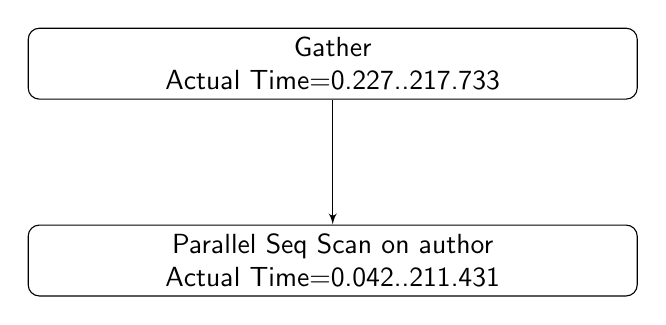
\begin{tikzpicture}[node distance=2.5cm, auto]

        % Styles for nodes
        \tikzset{
            base/.style={draw, align=center, minimum height=4ex, fill=white, font=\sffamily},
            block/.style={base, rectangle, text width=7.5cm, minimum height=2em, rounded corners},
            line/.style={draw, -latex'}
        }
    
        % Nodes
        \node [block] (gather) {Gather\\
                                Actual Time=0.227..217.733};
        \node [block, below of=gather] (parallelscan) {Parallel Seq Scan on author\\
                                                       Actual Time=0.042..211.431};
    
        % Lines
        \draw [line] (gather) -- (parallelscan);
    
    \end{tikzpicture}
\end{center}

计划是最优的,因为目前已经建立了关于name的索引。

\subsubsection{测试语句二}

根据作者姓名(模糊)搜索其撰写的文献:
\begin{lstlisting}[language=sql]
EXPLAIN ANALYZE SELECT w.author_name, ar.id, ar.title, ar.abstract, ar.doi, ar.license, ar.publish_time, ar.url
FROM "write" w
JOIN article ar ON w.article_id = ar.id
WHERE w.author_name LIKE '%' || 'aa' || '%';
\end{lstlisting}

这里我们将作者姓名的模糊搜索条件改为了'aa'。

得到结果:

\begin{lstlisting}
Gather  (cost=1000.55..497960.17 rows=155110 width=752) (actual time=5.822..4216.708 rows=81596 loops=1)
  Workers Planned: 2
  Workers Launched: 2
  ->  Nested Loop  (cost=0.56..481449.17 rows=64629 width=752) (actual time=5.800..3968.465 rows=27199 loops=3)
        ->  Parallel Seq Scan on write w  (cost=0.00..225212.96 rows=64629 width=40) (actual time=5.601..875.663 rows=27199 loops=3)
              Filter: ((author_name)::text ~~ '%aa%'::text)
              Rows Removed by Filter: 5279998
        ->  Index Scan using idx_article_id on article ar  (cost=0.56..3.96 rows=1 width=740) (actual time=0.113..0.113 rows=1 loops=81596)
              Index Cond: ((id)::text = (w.article_id)::text)
Planning Time: 1.835 ms
JIT:
  Functions: 24
  Options: Inlining false, Optimization false, Expressions true, Deforming true
  Timing: Generation 1.289 ms, Inlining 0.000 ms, Optimization 0.777 ms, Emission 15.827 ms, Total 17.893 ms
Execution Time: 4242.602 ms
\end{lstlisting}

可以看到耗时4242.602 ms。

由此,可以画出执行计划树,每个节点的功能和执行时间等信息由图所示:

\begin{center}
    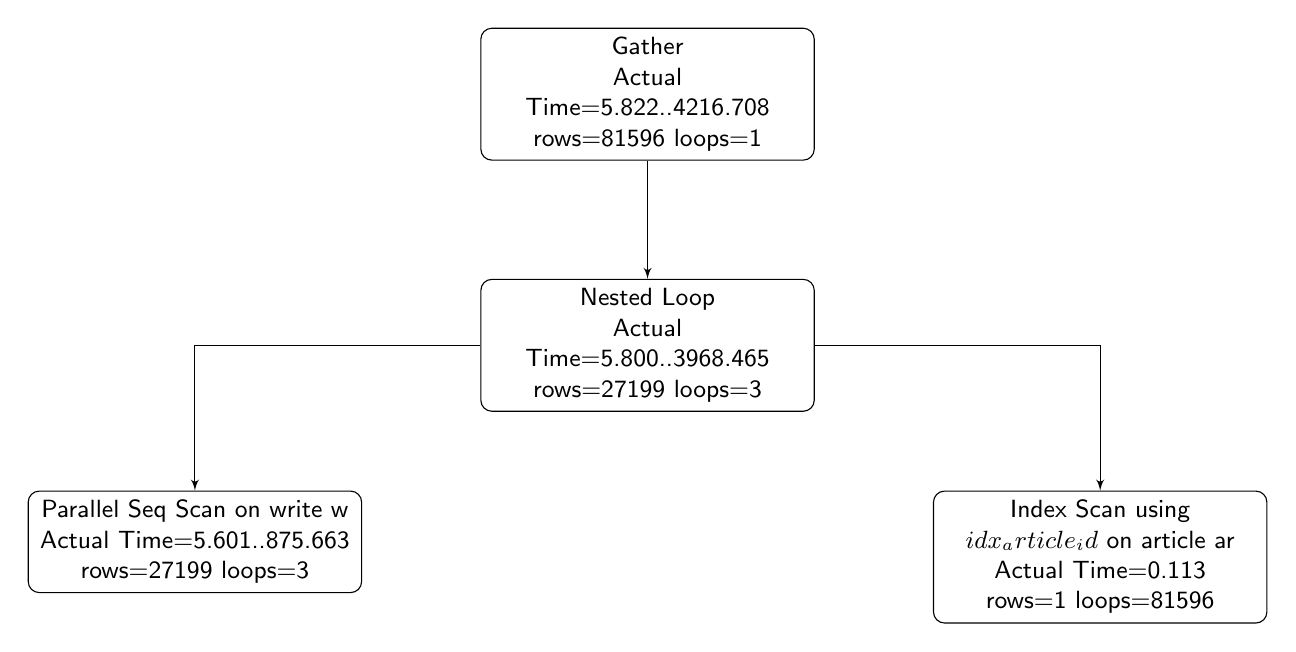
\begin{tikzpicture}[node distance=1.5cm, auto, font=\sffamily\small]

        % Styles for nodes
        \tikzset{
            base/.style={draw, align=center, minimum height=4ex, fill=white},
            block/.style={base, rectangle, text width=4cm, minimum height=2em, rounded corners},
            line/.style={draw, -latex'}
        }
    
        % Nodes
        \node [block] (gather) {Gather\\
                                Actual Time=5.822..4216.708 rows=81596 loops=1};
        \node [block, below=of gather] (nestedloop) {Nested Loop\\
                                                      Actual Time=5.800..3968.465 rows=27199 loops=3};
        \node [block, below left=1cm and 1.5cm of nestedloop] (parallelscan) {Parallel Seq Scan on write w\\
                                                                             Actual Time=5.601..875.663 rows=27199 loops=3};
        \node [block, below right=1cm and 1.5cm of nestedloop] (indexscan) {Index Scan using $idx_article_id$ on article ar\\
                                                                            Actual Time=0.113 rows=1 loops=81596};
    
        % Lines
        \draw [line] (gather) -- (nestedloop);
        \draw [line] (nestedloop) -| (parallelscan);
        \draw [line] (nestedloop) -| (indexscan);
    
    \end{tikzpicture}
\end{center}

计划是最优的。在完成本实验前,我们已经对article和write表建立了关于article\_id和author\_name的索引。

\subsubsection{测试语句三}

根据文献标题(模糊)搜索文献信息:
\begin{lstlisting}[language=sql]
SELECT id, title, abstract, doi, license
FROM (
  SELECT * 
  FROM article
  WHERE title LIKE '%e%'
) AS art
JOIN publish ON id = publish.article_id
JOIN write ON id = write.article_id;
\end{lstlisting}

这里我们将文献标题的模糊搜索条件改为了'e'。

得到结果:

\begin{lstlisting}
Merge Join  (cost=1.99..1655239.48 rows=15858854 width=633) (actual time=59.589..12196.366 rows=15979725 loops=1)
  Merge Cond: ((article.id)::text = (write.article_id)::text)
  ->  Merge Join  (cost=1.37..1068038.09 rows=3395082 width=663) (actual time=59.573..7377.889 rows=3409388 loops=1)
        Merge Cond: ((article.id)::text = (publish.article_id)::text)
        ->  Index Scan using idx_article_id on article  (cost=0.56..878208.40 rows=3373627 width=633) (actual time=59.540..4803.104 rows=3397735 loops=1)
              Filter: (title ~~ '%e%'::text)
              Rows Removed by Filter: 19808
        ->  Index Only Scan using idx_publish_arid on publish  (cost=0.56..139086.18 rows=3429273 width=30) (actual time=0.019..460.099 rows=3429428 loops=1)
              Heap Fetches: 705
  ->  Index Only Scan using idx_write_aeid on write  (cost=0.56..380331.80 rows=15917336 width=28) (actual time=0.008..1508.872 rows=16048677 loops=1)
        Heap Fetches: 1278
Planning Time: 0.799 ms
JIT:
  Functions: 10
  Options: Inlining true, Optimization true, Expressions true, Deforming true
  Timing: Generation 0.570 ms, Inlining 5.711 ms, Optimization 33.263 ms, Emission 20.551 ms, Total 60.095 ms
Execution Time: 12666.721 ms
\end{lstlisting}

可以看到耗时12666.721 ms。

由此,可以画出执行计划树,每个节点的功能和执行时间等信息由图所示:



\begin{center}
    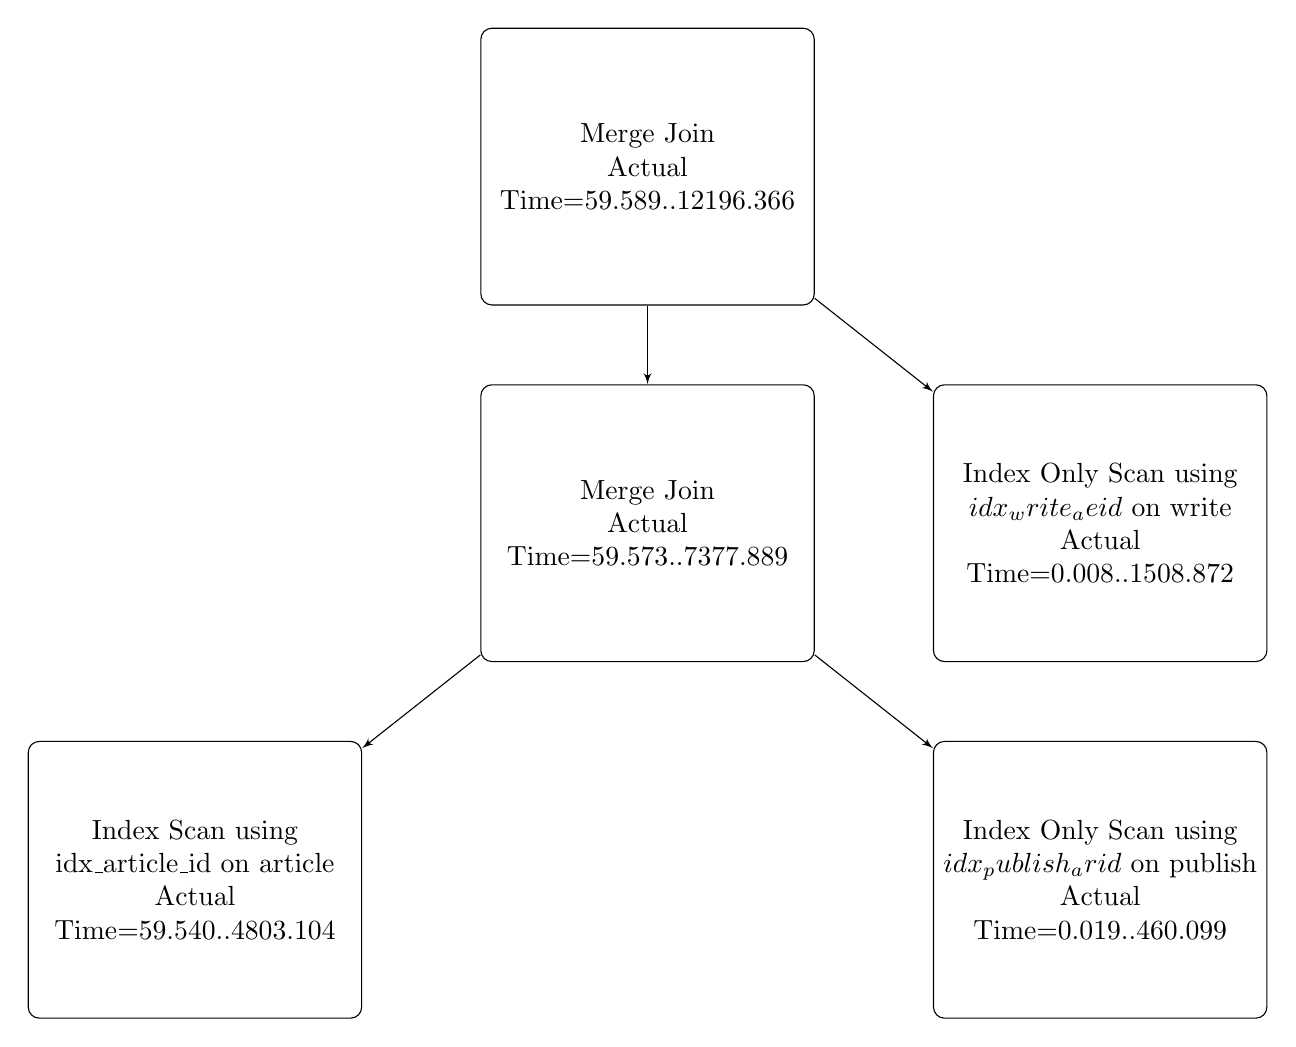
\begin{tikzpicture}
        % Nodes
        \node [block] (mergejoin1) {Merge Join\\
                                    Actual Time=59.589..12196.366};
        \node [block, below=of mergejoin1] (mergejoin2) {Merge Join\\
                                                          Actual Time=59.573..7377.889};
        \node [block, below left=1cm and 1.5cm of mergejoin2] (indexscan1) {Index Scan using idx\_article\_id on article\\
                                                                            Actual Time=59.540..4803.104};
        \node [block, below right=1cm and 1.5cm of mergejoin2] (indexonlyscan1) {Index Only Scan using $idx_publish_arid$ on publish\\
                                                                                 Actual Time=0.019..460.099};
        \node [block, below right=1cm and 1.5cm of mergejoin1] (indexonlyscan2) {Index Only Scan using $idx_write_aeid$ on write\\
                                                                                 Actual Time=0.008..1508.872};
    
        % Lines
        \draw [line] (mergejoin1) -- (mergejoin2);
        \draw [line] (mergejoin1) -- (indexonlyscan2);
        \draw [line] (mergejoin2) -- (indexscan1);
        \draw [line] (mergejoin2) -- (indexonlyscan1);
    
    \end{tikzpicture}

\end{center}

计划是最优的。在完成本实验前,我们已经对article、publish和write表建立了关于article\_id,article\_name的索引。

\section{存在的问题及解决方案}

在本次实验中,我们对数据库的性能进行了测试,发现了一些问题,比如有的查询耗时较长,有的查询执行计划不够优化等。对于这些问题,我们都可以通过建立索引来加速查询。

\section{实验总结}

在老师和助教老师的帮助下,我们了解了索引在数据库中的作用,以及索引对数据库性能的影响。通过实验,我们对索引的作用有了更深入的理解。在实验中,我们对TPCH测试语句和课程项目SQL语句进行了测试,通过测试,我们发现了一些问题,并对这些问题提出了解决方案;通过实验,我们对数据库的性能有了更深入的了解。

\end{document}